\documentclass[12pt]{report}

\setlength{\topmargin}{0.0in}
\setlength{\oddsidemargin}{0.33in}
\setlength{\textheight}{9.0in}
\setlength{\textwidth}{6.0in}
\renewcommand{\baselinestretch}{1.25}

\usepackage{nicematrix}
\usepackage{multicol}
\usepackage{caption}
%\usepackage[margin=0.75in]{geometry}
\usepackage[edges]{forest}
\usepackage{graphicx,wrapfig,lipsum}
\usepackage{amsmath,empheq}
\usepackage{dirtree}
\usepackage{titlesec}
\usepackage{breqn}
\setcounter{secnumdepth}{4}
\titleformat{\paragraph}
{\normalfont\normalsize\bfseries}{\theparagraph}{1em}{}
\titlespacing*{\paragraph}
{0pt}{3.25ex plus 1ex minus .2ex}{1.5ex plus .2ex}
\usepackage{amssymb}
\usepackage{amsthm}
\usepackage[style=numeric,backend=biber]{biblatex}
\addbibresource{bibliographydiss.bib}
\usepackage{tikz}
\def\checkmark{\tikz\fill[scale=0.4](0,.35) -- (.25,0) -- (1,.7) -- (.25,.15) -- cycle;}
\usepackage[utf8]{inputenc}
\usepackage[english]{babel}
\usepackage{hyperref}
\usepackage[ruled]{algorithm2e}
\usepackage{amssymb}
\usepackage{graphicx}
\usepackage{cancel}
\usepackage{epstopdf}
\usepackage{mathtools}
\usepackage{float}
\usepackage{caption}
\usepackage{subcaption}
\usepackage{setspace}
\usepackage{bm}
\usepackage[export]{adjustbox}
\usepackage{relsize}
\usepackage{listings}
\usepackage[toc,page]{appendix}
\usepackage{cancel}

\title{Effects of Distributed Delay on Turing Pattern Formation in Reaction-Diffusion Systems.}
\author{Alec Sargood}
\begin{document}
\date{2021}
\maketitle

\tableofcontents
\newpage
\chapter{Introduction}

\section{Background}

Morphogenesis is a complex spatio-temporal process responsible for the development of cellular shape or form, for example, the controlling the spatial distribution of cells during the development process of an embryo, or the growth of cancerous tissue \cite{morph}. In 1952 \cite{turing}, Turing proposed that the morphogenesis process could be mathematically modelled as a purely chemical basis via the interaction of morphogens, or reactants, whose evolutions are described by a system of coupled reaction-diffusion equations. Turing's models have been used to explain the apparent self-organisation of cells leading to naturally occurring pattern formation, such as on animal coats (e.g. spots on a jaguar \cite{painter}), the formation of features (e.g. pattern of feathers on birds \cite{bailleul}), and in developmental biology (e.g. vertebrate limb development \cite{miura1,glimm,miura2}). It was proposed that a stable steady-state, robust to small perturbations in the spatially homogeneous setting, could become unstable and sensitive to small perturbations with the introduction of diffusion, leading to spatially inhomogeneous patterns. Physically, the spatially homogeneous state can be thought of as representing early stages of development, e.g a zygote with negligible domain size. The diffusion term therefore acts as a transportation mechanism for the reactants across a suffiently large spatial domain resulting in cellular development of shape and form. In the example of the zygote, cellular division results in a non-neglible spatial domain, and the diffusion of chemicals across the pool of cells culminates in embroygenesis - the process by which an embryo takes its specifc shape or form.
\\
Morphogenesis relies on the ability of cells to adopt a state appropriate to their temporal and spatial position \cite{gaffmonk}. The mechanism allowing cells to adopt an appropriate state is known as differential gene expression, and depends tightly on the communication between cells, achieved through cellular signalling. Typical reaction-diffusion systems assume a neglibible timescale on which the cellular signalling and gene expression processes occur. The gene expression process is however extremely complex and proceeds through several stages \cite{gaffmonk}, namely gene transcription and gene translation. These sub-processes can take large amounts of time, and it has been experimentally shown that these time delays are typically on the order of minutes, but in some cases can be as large as a few hours \cite{gaffmonk,tennyson}. These time delays can therefore be on the same order of magnitude as the pattern formation process itself. For example, the basic body plan of a zebrafish is established in less than 24 hours \cite{gaffmonk,kimmel}. It is therefore important to consider these delays when studying pattern formation in Turing mechanisms.
\\
Such time delays have been investigated in the context of Turing patterns \cite{gaffmonk,leegaffney,yigaffneyli,jiang,leegaffmonk,bratsun,william}, by incorporating fixed constant delays into the models. Typical reaction-diffusion models that have been considered include the Schnakenberg model and it's time-delayed variants \cite{schnakenberg}, and the Gierer-Meinhardt model \cite{gm}. The numerical results in \cite{gaffmonk}, which studied the ligand-internalisation (LI) variant of the Schnakenberg model, showed that the time taken until pattern formation occurs drastically increases as the gene expression time delay in the model is increased, and that small delays can cause a large increase in time-to-pattern. Numerical simulations on a growing domain also suggested that time delay can cause a failure in Turing pattern formation. Similar results have also been discussed in \cite{leegaffney,leegaffmonk}, for both the LI and reverse-ligand bonding (RLB) variants of the Schnakenberg model, where simulations have shown the disruption time delay can cause to pattern formation, as well as inducing temporal oscillations and increasing sensitivity of Turing instabilities to initial conditions. An analytical study of time delay in \cite{yigaffneyli} for the LI and RLB models has shown that increasing time delay can antagonise the the induction of Turing patterns. The work in \cite{jiang} showed a vast range of possible behaviours obtainable in the RLB model, including both spatial and temporal oscillations. It has therefore in general been found that these time delays can increase the time taken until pattern formation occurs, induce oscillations, or completely prevent pattern formation, and therefore pose a potential obstacle to applying Turing models to real systems. Interestingly, more recently it has been observed in \cite{fadai} that introducing time-delay in only the activator term of the reaction-diffusion mechanism for the Gierer-Meinhardt model can act as a stabilising agent for pattern formation and increase the parameter space where one might expect to find Turing patterns, compared to a no-delay model. This is a result we look to explore in our report.
\\
In reality however, the biological process responsible for gene expression, namely gene transcription and gene translation, are inherintly stochastic \cite{raj,elowitz,mcadams,paulsson}. Introducing merely a fixed-delay term into the kinetic equations is an oversimplification of the underlying biological process on a cellular level, and leads us to consider a distribution of time delays at the macroscopic level \cite{bratsun,krausenew}. In this report we are interested in whether implementing different forms of the delay, namely distributed delay, can alleviate some of the problems caused by the fixed delay case. We will first outline some of the mathematical preliminaries used throughout this paper, including an outline of Turing pattern theory, and the numerical methods we use.
Chapter 2 will be concerned with verifying and extending the numerical results in current literature concerned with the fixed delay model, as well as looking at the presented theory in more depth. We will specifically be concerned with evaluating the robustness of current results to varying initial and boundary conditions. We also aim to analytically show the relationship between a fixed time-delay, and the time taken for pattern formation to occur. Finally, Chapter 3 will focus on the distributed delay model. We aim to produce novel linear analysis for the distributed delay case and numerically verify any observations we make.

\section{Preliminaries}
\subsection{Model Introduction}
The mathematical model we will consider is the Schnakenberg model \cite{schnakenberg} - one of the simplest `toy' models that exhibit some of the key behaviours that we are interested in, as well as one that has been studied extensively in the context of fixed time delays. The model describes the evolution and interaction between two reactants, $u$ and $v$. Only considering two reactants is a gross simplification of the biological process on a cellular level, but it is still a non-trivial case than can admit Turing patterns. In this report, we restrict our investigation to one spatial domain. The non-dimensionalised model description we use is motivated from \cite{gaffmonk} and is given by

\begin{equation}\label{system}
    \begin{split}
    \frac{\partial u}{\partial t}&=D_u\frac{\partial^2 u}{\partial x^2}+f(u,v),\\
    \frac{\partial v}{\partial t}&=D_v\frac{\partial^2 v}{\partial x^2}+g(u,v) \quad\quad\quad x\in\Omega,
    \end{split}
\end{equation}
where $\Omega$ is the spatial domain, which we consider here as $\Omega=[0,L]$, for some domain length $L\in\mathbb{R}_{>0}$. Since we are interested in the pattern formation arising from the self-organisation of cells, we implement no flux (homogeneous Neumann) boundary conditions on the boundary of the spatial domain $\partial\Omega$, namely $\frac{\partial u}{\partial x}=\frac{\partial v}{\partial x}=0$ at $x=0, L$. We also assume initial conditions $u(x,0)$ and $v(x,0)$ are given. $D_u$ and $D_v$ are the diffusive coefficients of the morphogens $u$ and $v$ respectively, and usually the ratio $D_u/D_v\ll1$.
The functions $f$ and $g$ are the functions describing the intrinsic chemical reaction between the two morphogens $u$ and $v$, and for the Schnakenberg model are given as
\begin{equation}
    \begin{split}
        f(u,v)&=a-u+u^2v\\
        g(u,v)&=b-u^2v,
    \end{split}
\end{equation}
for parameters $a$ and $b$.
As typical when studying Turing patterns, initial conditions will be chosen as a small random perturbation from the spatially homogeneous steady state, found as the roots of $f$ and $g$. Further details on the model parameters $(a,b)$ can be found in \cite{gaffmonk}. Importantly, necessary conditions on $(a,b)$ and the ratio $D_u/D_v$ can be found for Turing pattern formation to occur. Unless otherwise stated, following the model description in \cite{gaffmonk}, we take $D_u=\epsilon^2/\gamma$ and $D_v=1/\gamma$, with $\epsilon^2=0.001$ and $\gamma=0.05$.


\subsection{Turing Pattern Formation Without Delay}

Here we give a brief overview of the mathematical theory underpinning Turing's mechanism, closely following the description in \cite{murray}. For further details, the reader should consult \cite{murray,beentjes}. Turing patterns occur when the spatially homogeneous stable steady-state becomes unstable in the presence of diffusion. We therefore first consider the spatially homogeneous model, and explore conditions necessary for the steady-state to be stable. In the case of the Schnakenberg model, the single steady-state, $(u_\star, v_\star)$, occurs at $(u_\star, v_\star)=\left(a+b, \frac{b}{(a+b)^2}\right)$. Since $a,b>0$, we have $u_\star,v_\star>0$ which is physically feasible. Following the methodology in \cite{murray}, we perform linear stability analysis. Taking a small perturbation from the steady-state, so that $\hat{u}=u-u_\star$, $\hat{v}=v-v_\star$ for $|\hat{u}|, |\hat{v}|<<1$, we consider the evolution of the perturbation. Denoting $\hat{\textbf{u}}$ as the vector of perturbations, $\hat{\textbf{u}}=\begin{bmatrix}\hat{u} \\ \hat{v}\end{bmatrix}$, the linearised system of \eqref{system} is given as
\begin{equation}\label{linsys}
\frac{\text{d}\hat{\textbf{u}}}{\text{dt}}=\textbf{J}_{(u_\star,v_\star)}\hat{\textbf{u}},
\end{equation}
where $\textbf{J}_{(u_\star,v_\star)}$ is the Jacobian matrix of the kinetic equations evaluated at the steady-state. Namely,
$$
\textbf{J}_{(u_\star,v_\star)}=\begin{pmatrix}f_u&f_v\\g_u&g_v\end{pmatrix}\Bigg|_{(u_\star,v_\star)}.
$$
The notation $f_u$ is used to denote the partial derivatve of $f$ with respect to $u$. Solutions of \eqref{linsys} are of the form
$$
\hat{\textbf{u}}\propto e^{\lambda t},
$$
for eigenvalues $\lambda$ of $J_{(u_\star,v_\star)}$. The steady-state is asympotically stable if the perturbation decays.
Denoting $\text{spec}(\textbf{M})$ as the set of eigenvalues of some matrix $\textbf{M}$, asympotica stability occurs when $\Re(\lambda)<0 \ \text{for all }\lambda\in \text{spec}(\textbf{J}_{(u_\star,v_\star)})$. However, if there exists $\lambda\in \text{spec}(\textbf{J}_{(u_\star,v_\star)}): \Re(\lambda)>0$,
then the pertubation will grow with time and the steady-state in unstable. The sum and product of the eigenvalues of $\textbf{J}_{(u_\star,v_\star)}$
are given by $\text{Tr}(\textbf{J}_{(u_\star,v_\star)})$ and $\text{det}(\textbf{J}_{(u_\star,v_\star)})$ respectively. The required conditions for stability are therefore
\begin{equation}\label{cond1}
    \begin{split}
\text{Tr}(\textbf{J}_{(u_\star,v_\star)})<0 &\implies f_u+g_v<0, \\
\text{det}(\textbf{J}_{(u_\star,v_\star)})>0 &\implies f_ug_v-f_vg_u>0,
\end{split}
\end{equation}
where the derivatives are evaluated at the steady-state $(u_\star,v_\star)$.
We now consider the full diffusive model and look for necessary conditions such that the previously stable steady-state is driven to instability. The linearised system is given by
\begin{equation}\label{linsys2}
    \frac{\partial \hat{\textbf{u}}}{\partial t}=\left[\textbf{D}\nabla^2+\textbf{J}_{(u_\star,v_\star)} \right]\hat{\textbf{u}},
\end{equation}
where $\textbf{D}=\begin{pmatrix}\epsilon^2/\gamma&0\\0&1/\gamma\end{pmatrix}$ is the matrix containing the diffusion coefficients of reactants.
The solution to the spatially dependent eigenvalue problem can be written as a linear combination of the eigenfunctions $w_k$ that satisfy the problem
\begin{equation}\label{eigprob}
\nabla^2w_k=-k^2w_k,\quad \quad \frac{\partial w_k}{\partial \textbf{n}}=0\text{ for } \textbf{x}\in\partial\Omega.
\end{equation}
We consider here only a regular 1D domain $\Omega=[0,L]$ for some domain length $L\in\mathbb{R}_{>0}$. We also note here that on a regular 1D domain $\Omega=[0,L]$ with no flux boundary conditions, $\frac{\partial w_k}{\partial \textbf{n}}=0\text{ for } \textbf{x}\in\partial\Omega$, the eigenfunctions will be of the form $w_k=\cos(k\pi x/L)$. $\partial\Omega$ denotes the boundary of the domain, and $\textbf{n}$ denotes the outward-facing normal.
We thus look for solutions to \eqref{linsys2} of the form
\begin{equation}\label{perturbgrow}
    \hat{\textbf{u}}=\sum_k \textbf{c}_ke^{\lambda_k t}w_k(\textbf{x}),
\end{equation}
where the constants $\textbf{c}_k$ are determined by using a Fourier expansion of the initial conditions in terms of the eigenfunctions $w_k$. $\lambda_k$ is the eigenvalue which determines the rate of temporal growth for each mode $k$, and thus determines whether a particular mode of pattern will be unstable and grow. Substituting this form into \eqref{linsys2}, along with using \eqref{eigprob} and simplifying, we obtain, for each $k$
$$
\lambda_k w_k=\textbf{J}w_k-\textbf{D}k^2w_k \implies (\lambda_k \textbf{I}-\textbf{J}+k^2\textbf{D})w_k=\textbf{0},
$$
with $\textbf{I}$ the identity matrix. Looking for non-trivial solutions for $w_k$, we set solve for roots of the characteristic polynomial, namely $\text{det}(\lambda_k \textbf{I}-\textbf{J}+k^2\textbf{D})=0$, which yields a quadratic equation for eigenvalues $\lambda_k(k)$ as a function of $k$. Finding roots of this quadratic such that $\Re(\lambda_k(k))>0$ for some $k\neq0$, we can conclude two necessary conditions for the instability of the steady-state in the presence of diffusion, namely
\begin{equation}\label{cond2}
    \begin{split}
    \frac{1}{\epsilon^2}f_u+g_v>0&\\
    \left(\frac{1}{\epsilon^2}f_u+g_v\right)^2-\frac{4}{\epsilon^2}(f_ug_v-f_vg_u)>0.
\end{split}
\end{equation}
We therefore have four necessary conditions in terms of $(a,b,\epsilon^2)$ for Turing patterns to occur. These conditions are only necessary, and not sufficient, as conditions \eqref{cond2} are only strictly valid in the limit $L\to\infty$. The larger the domain size $\Omega=[0,L]$ we consider, the better the approximation the conditions will be. Using the first two conditions in \eqref{cond1}, a bifurcation diagram in the $(a,b)$ parameter space can be plotted showing the regions corresponding to a stable or unstable steady state. This can be seen in figure \ref{fig:bifsh}. Using the additional conditions in \eqref{cond2} and the fixed value $\epsilon^2=0.001$, the parameter region in the $(a,b)$ parameter space in which Turing patterns can occur can also be plotted. This `Turing space' can be seen in figure \ref{fig:turingspace}.

\begin{figure}[H]
    \centering
    \begin{subfigure}[b]{0.45\textwidth}
        \centering
        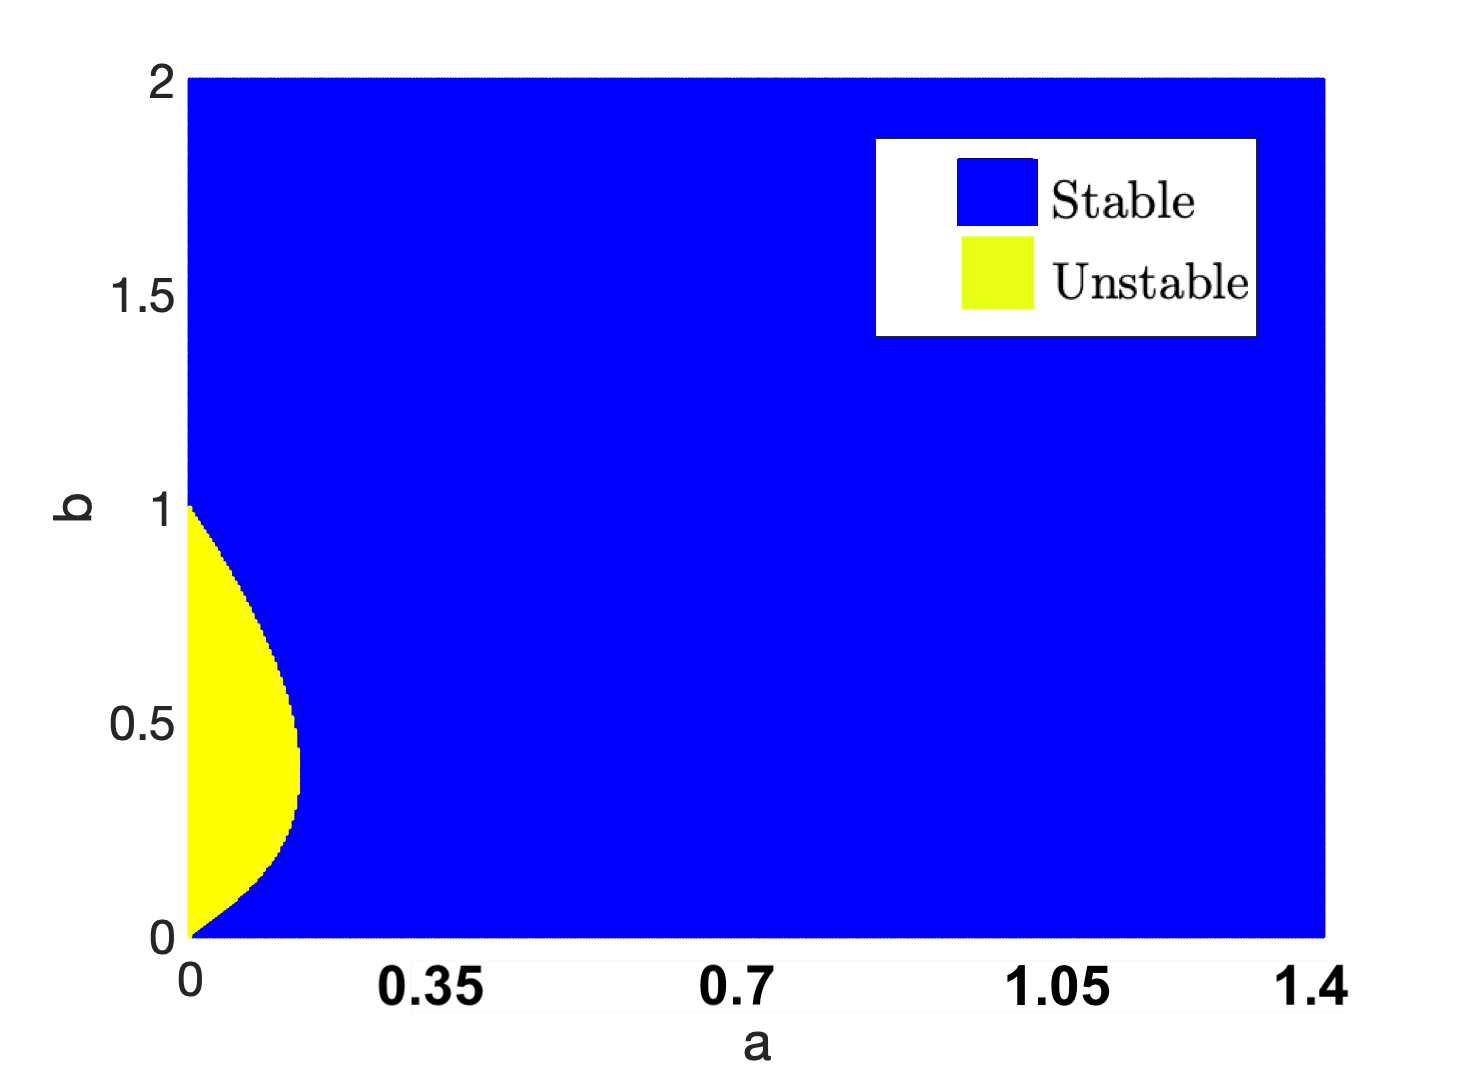
\includegraphics[width=8cm,height = 6cm]{bifsh.png}
        \caption{Bifurcation diagram for spatially homogeneous model, no delay.}
        \label{fig:bifsh}
    \end{subfigure}
    \hfill
    \begin{subfigure}[b]{0.45\textwidth}
        \centering
        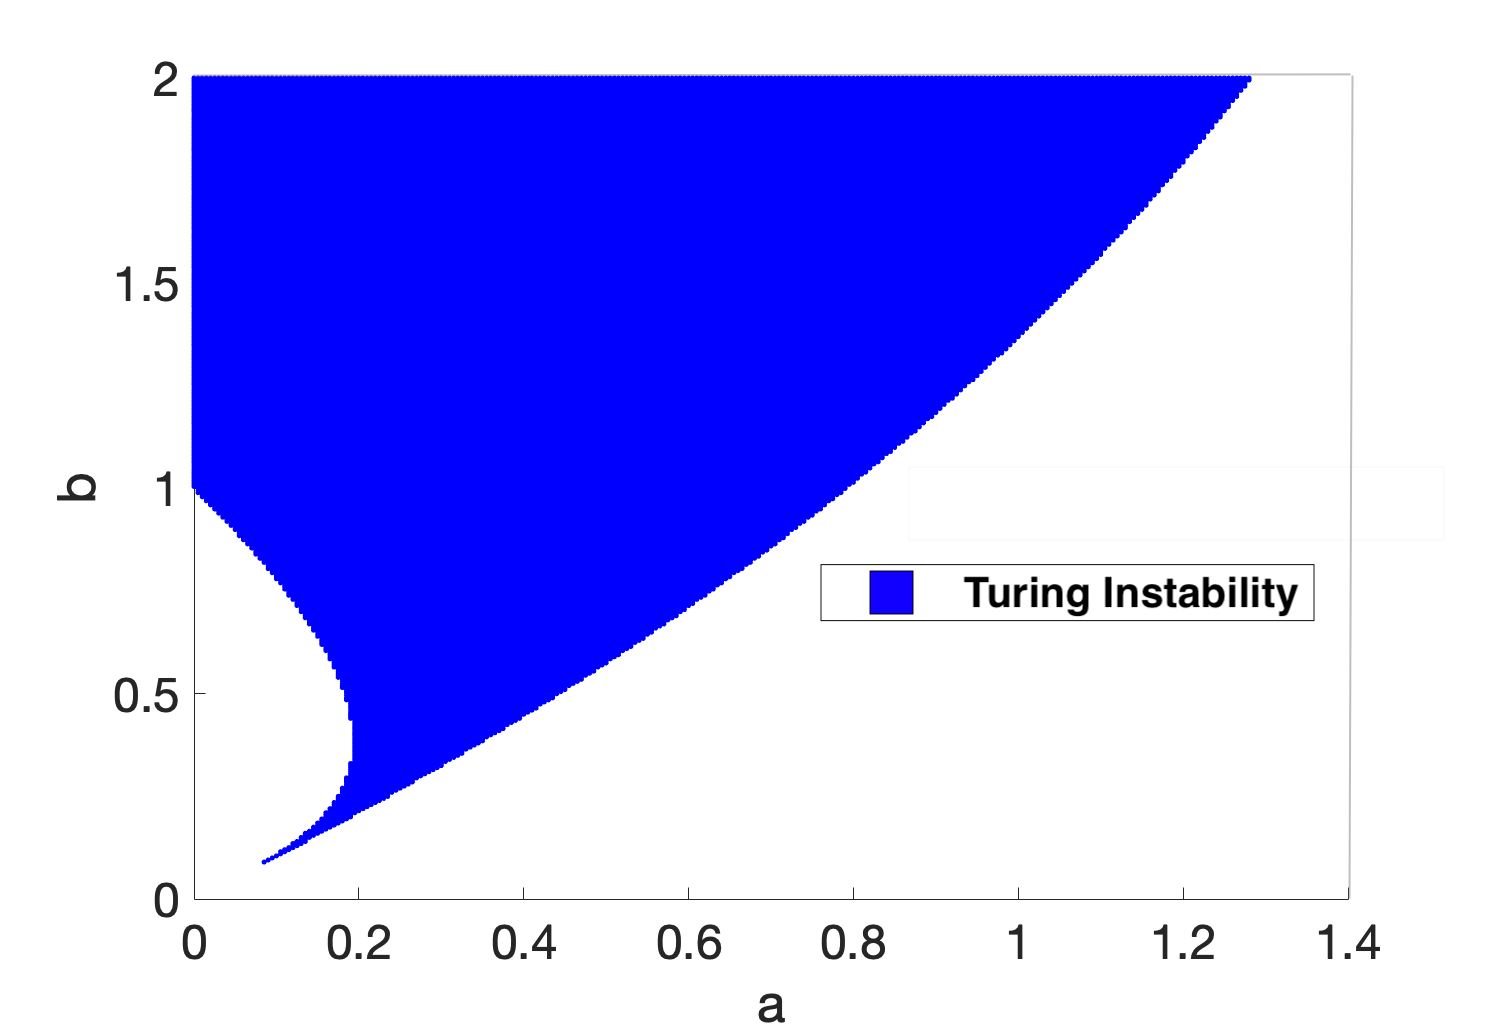
\includegraphics[width=8cm,height = 6cm]{turingspace.png}
        \caption{Turing space, no delay.}
        \label{fig:turingspace}
    \end{subfigure}
    \caption{}
    \label{fig:dispfixed}
\end{figure}

\subsection{Numerical Implementation}\label{section:numimp}
\subsubsection{Spatial Discretisation}
In order to numerically resolve the spatial derivatives $\frac{\partial^2 u}{\partial x^2}$, $\frac{\partial^2 v}{\partial x^2}$ and implement the relevant boundary conditions, a finite-difference scheme is used. We use $m=500$ equally spaced spatial discretisation points on the domain $x\in\Omega=[0,L]$, with the spatially discretised points given as $\textbf{x}=[x_1,\cdots,x_m]^T$ where $x_i=(i-1)\Delta x$, with $\Delta x=\frac{L}{m-1}$. This ensures $x_1=0$ and $x_m=L$. Letting $U_i^t$ denote the numerical approximation to $u(x_i,t)$, we use a second-order central difference approximation \cite{finitediff} to evaluate the second-order derivatve $\frac{\partial^2 u}{\partial x^2}(x_i,t)$. Namely,
\begin{equation}
\frac{\partial^2 u}{\partial x^2}(x_i,t)\approx\frac{1}{\Delta x^2}\left(U_{i+1}^t-2U_i^t+U_{i-1}^t\right).
\end{equation}
By denoting $\textbf{U}^t$ as the vector of numerical approximations to $u(x,t)$ at some time $t$ across the whole spatial domain $\textbf{x}$, so that $\textbf{U}^t=\left[U_1^t,\cdots,U_m^t\right]^T$, the numerical approximation of the second-order derivative across the whole spatial domain at some time $t$ can be computed in matrix form as
\begin{equation}
    \frac{\partial^2 u}{\partial \textbf{x}^2}\approx A\textbf{U}^t.
\end{equation}
$A$ is the discrete second-order differential operator, and is given by
\begin{equation}\label{A}
A=\frac{1}{\Delta x^2}\begin{bmatrix}
   -2&  1&  &  & 0\\
   1&  -2&  1&  & \\
   &  \ddots&  \ddots&  \ddots& \\
   &  &  1&  -2& 1\\
   0&  &  &  1& -2
  \end{bmatrix}.
\end{equation}
The sparse nature of $A$ allows for computational advantages when implementing the finite-difference scheme. In order to implement homogeneous Neumann boundary conditions, a first-order central difference approximation is used with `ghost' nodes appended at $x_{-1}$ and $x_{m+1}$. This results in altering entries $A_{1,2}$ and $A_{m,m-1}$ from a $1$ to a $2$, as seen in \eqref{Aneumann}. Further details on using `ghost' nodes can be found in appenix \ref{appendix:extramath}. To implement homogeneous Dirichlet conditions, the first and last rows of $A$ are set to $0$, as seen in \eqref{Adirichlet}. Since homogeneous Dirichlet conditions require $u(x)=0$ at $x=0,L$ for all $t>0$, we also set the initial conditions and kinetic functions to equal $0$ at the end nodes.
\begin{multicols}{2}
\begin{equation}\label{Aneumann}
    \begin{split}
A&=\frac{1}{\Delta x^2}\begin{bmatrix}
   -2&  2&  &  & 0\\
   1&  -2&  1&  & \\
   &  \ddots&  \ddots&  \ddots& \\
   &  &  1&  -2& 1\\
   0&  &  &  2& -2
  \end{bmatrix}.\\
  A &\textit{ with homogeneous Neumann conditions}
    \end{split}
\end{equation}
\break
\begin{equation}\label{Adirichlet}
    \begin{split}
A&=\frac{1}{\Delta x^2}\begin{bmatrix}
   -0&  0& \cdots &  & 0\\
   1&  -2&  1&  & \\
   &  \ddots&  \ddots&  \ddots& \\
   &  &  1&  -2& 1\\
   0&\cdots  &  &  0& 0
  \end{bmatrix}.\\
  A & \textit{ with homogeneous Dirichlet conditions}
    \end{split}
\end{equation}
\end{multicols}

\subsubsection{Temporal Discretisation}

\newpage
\chapter{Fixed Delay Model}

The time-delay form of the model we consider is the Ligand Internalistion (LI) variant of the standard Schnakenberg model. The LI model assumes that, a reaction at the cell surface is followed by internalisation of a morphogen, before the gene expression process can continue and morphogen production can occur \cite{leegaffney,yigaffneyli}. As derived in \cite{leegaffney}, the LI model is given by
\begin{equation}\label{fixed}
  \begin{split}
  \frac{\partial u}{\partial t}&=D_u\frac{\partial^2u}{\partial x^2}+a-u-2u^2v+3\hat{u}^2\hat{v} \text{ds}\\
  \frac{\partial v}{\partial t}&=D_v\frac{\partial^2v}{\partial x^2}+b-u^2v,
\end{split}
\end{equation}
where $u=u(x,t)$, $v=v(x,t)$ and $\hat{u}$, $\hat{v}$ are evaluated at some delay $\tau$, so that $\hat{u}=u(x,t-\tau)$ and $\hat{v}=v(x,t-\tau)$. The time-delay terms in the LI model only appear in the activator's dynamics. This is based on the assumption that the gene expression process, and thus the source of the time delay, is responsible for autocatalysis of the activator in the reaction-diffusion mechanism \cite{gaffmonk}.
\section{Linear Analysis}
Following the methodology in \cite{yigaffneyli}, we take a small perturbation about the steady-state $u(x,t)=u_\star+\epsilon\xi(x,t)$ and $v(x,t)=v_\star+\epsilon\eta(x,t)$, where $|\epsilon|\ll 1$. Taylor expanding up to $O(\epsilon)$ about the steady-state, the linearised dynamics of \eqref{fixed} are then given by

\begin{equation}\label{linfixed}
  \begin{split}
\frac{\partial\xi}{\partial t}&=D_u\frac{\partial^2\xi}{\partial x^2}-\xi-4u_\star v_\star\xi+6u_\star v_\star\hat{\xi}-2u_\star^2\eta+3u_\star^2\hat{\eta},\\
\frac{\partial\eta}{\partial t}&=D_v\frac{\partial^2\eta}{\partial x^2}-2u_\star v_\star\xi-u_\star^2\eta,
\end{split}
\end{equation}
with $\hat{\xi}=\xi(x,t-\tau)$ and $\hat{\eta}=\eta(x,t-\tau)$. Substituting into \eqref{linfixed} an ansatz of the form $\begin{pmatrix}\xi\\\eta\end{pmatrix}=\begin{pmatrix}\xi_0e^{-\lambda t}\cos(k\pi x)\\ \eta_0e^{-\lambda t}\cos(k\pi x)\end{pmatrix}$, we obtain the characteristic equation $D_k=0$ \cite{yigaffneyli}, given by,

\begin{equation}\label{characfix}
D_k=\lambda^2+\alpha_k\lambda+\beta_k+(\gamma_k\lambda+\delta_k)e^{-\lambda\tau}=0,
\end{equation}
where the coefficients are given by,\footnote{We note the coefficient of $\beta_k$ differs from that of \cite{yigaffneyli} due to a suspected error in the cited paper.}
\begin{align}
\alpha_k&=(D_u+D_v)k^2\pi^2+u_\star^2+4u_\star v_\star+1\\
\beta_k&=(D_v\pi^2k^2+u_\star^2)(D_u\pi^2k^2+4u_\star v_\star+1)-4u_\star^3v_\star\\
\gamma_k&=-6u_\star v_\star\\
\delta_k&=-6D_vu_\star v_\star k^2\pi^2.
\end{align}
This characteristic equation can be used to determine the parameter sets $(a,b,D_u,D_v,\tau)$ in which pattern formation occurs. From \eqref{perturbgrow}, the perturbation grows like $e^{\lambda t}\cos(k\pi x)$, and so if there exists a $k\neq0$ for a given $(a,b,D_u,D_v,\tau)$ such that $\Re(\max_k(\lambda))>0$, we expect pattern formation. To find the roots $\lambda(k)$ of $D_k$, the `marching sqaures' algorithm \cite{marchingsquares} in chebfun was used \cite{chebfun}. To do so, we split the characteristic equation \eqref{characfix} into it's real and imaginary parts $D_k^{\Re}$ and $D_k^{\text{Im}}$. These are given by

\begin{align}\label{realfix}
D_k^{\Re}&=x^2-y^2+\alpha_kx+\beta_k+e^{-x\tau}[\gamma_kx\cos(-y\tau)-\gamma_ky\sin(-y\tau)+\delta_k\cos(-y\tau)],\\
D_k^{\text{Im}}&=2xy+\alpha_ky+e^{-x\tau}[\gamma_kx\sin(-y\tau)+\gamma_ky\cos(-y\tau)+\delta_k\sin(-y\tau)].\label{complexfix}
\end{align}

Figure \ref{fig:dispfixed}  show $\max_k(\Re(\lambda))$ plotted against $\tau$, for multiple given $(a,b)$ parameter sets. These plots were produced by varying $k$ over $[0,20]$ at regular discrete intervals for a given $\tau$, and for each $k$, the roots of \eqref{realfix} and \eqref{complexfix} computed. The maximum over the $k$ of the $\Re(\lambda)$ was taken, and then repeated over a varying $\tau$. The time-delay $\tau$ was varied over $[0,1]$ at regular intervals of $0.1$.

\begin{figure}[H]
    \centering
    \begin{subfigure}[b]{0.45\textwidth}
        \centering
        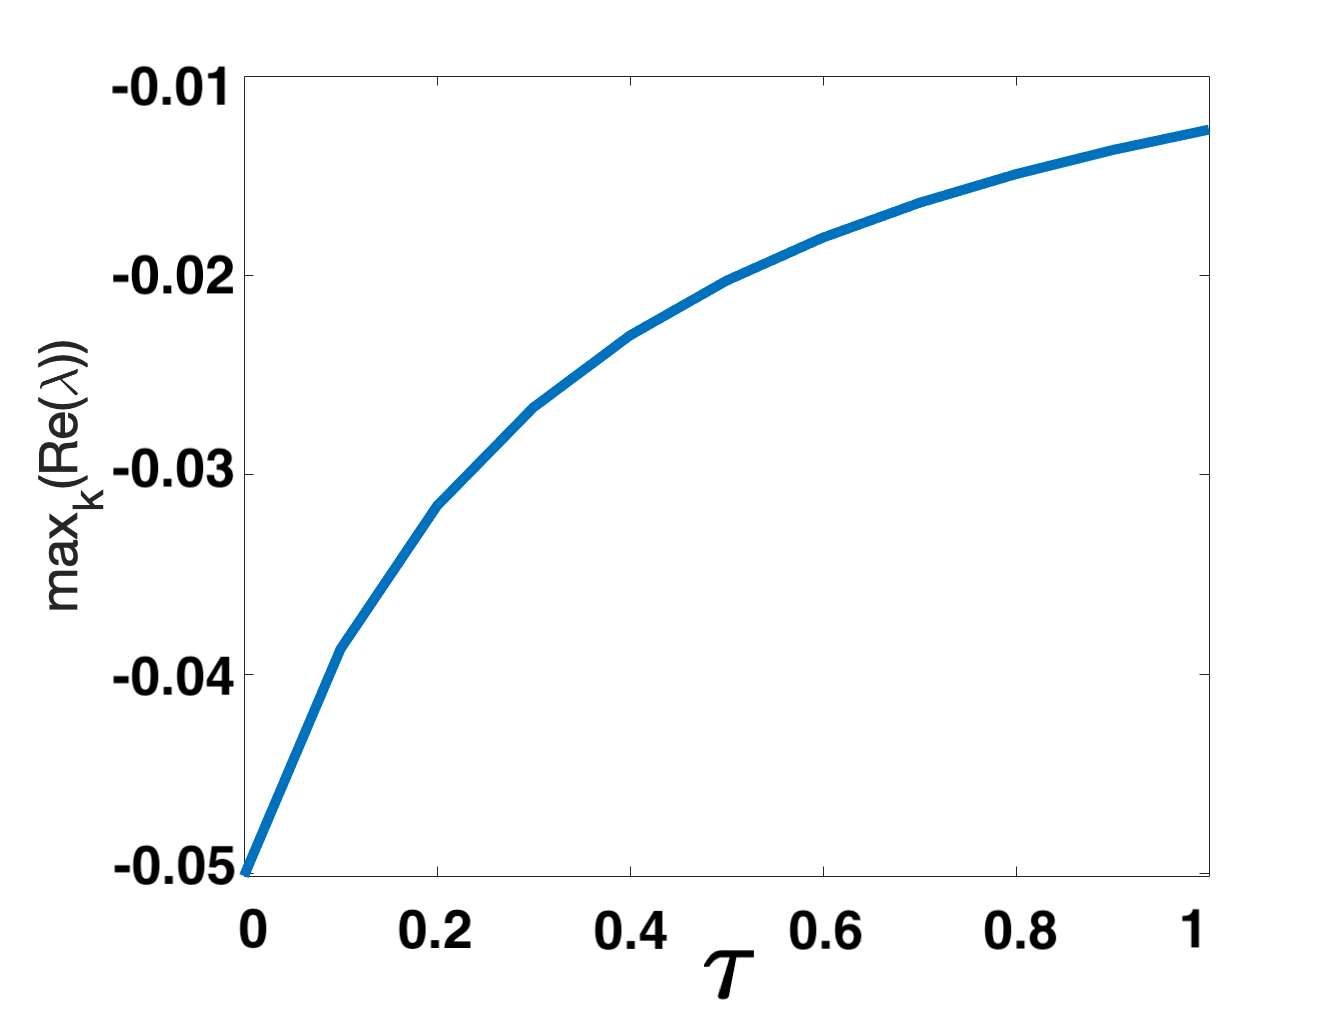
\includegraphics[width=8cm,height = 6cm]{disp1.png}
        \caption{$(a,b)=(0.4,0.4)$. $\max_k(\Re(\lambda))<0 \quad \forall\tau\in[0,1]$. Linear theory predicts no pattern formation. }
        \label{}
    \end{subfigure}
    \hfill
    \begin{subfigure}[b]{0.45\textwidth}
        \centering
        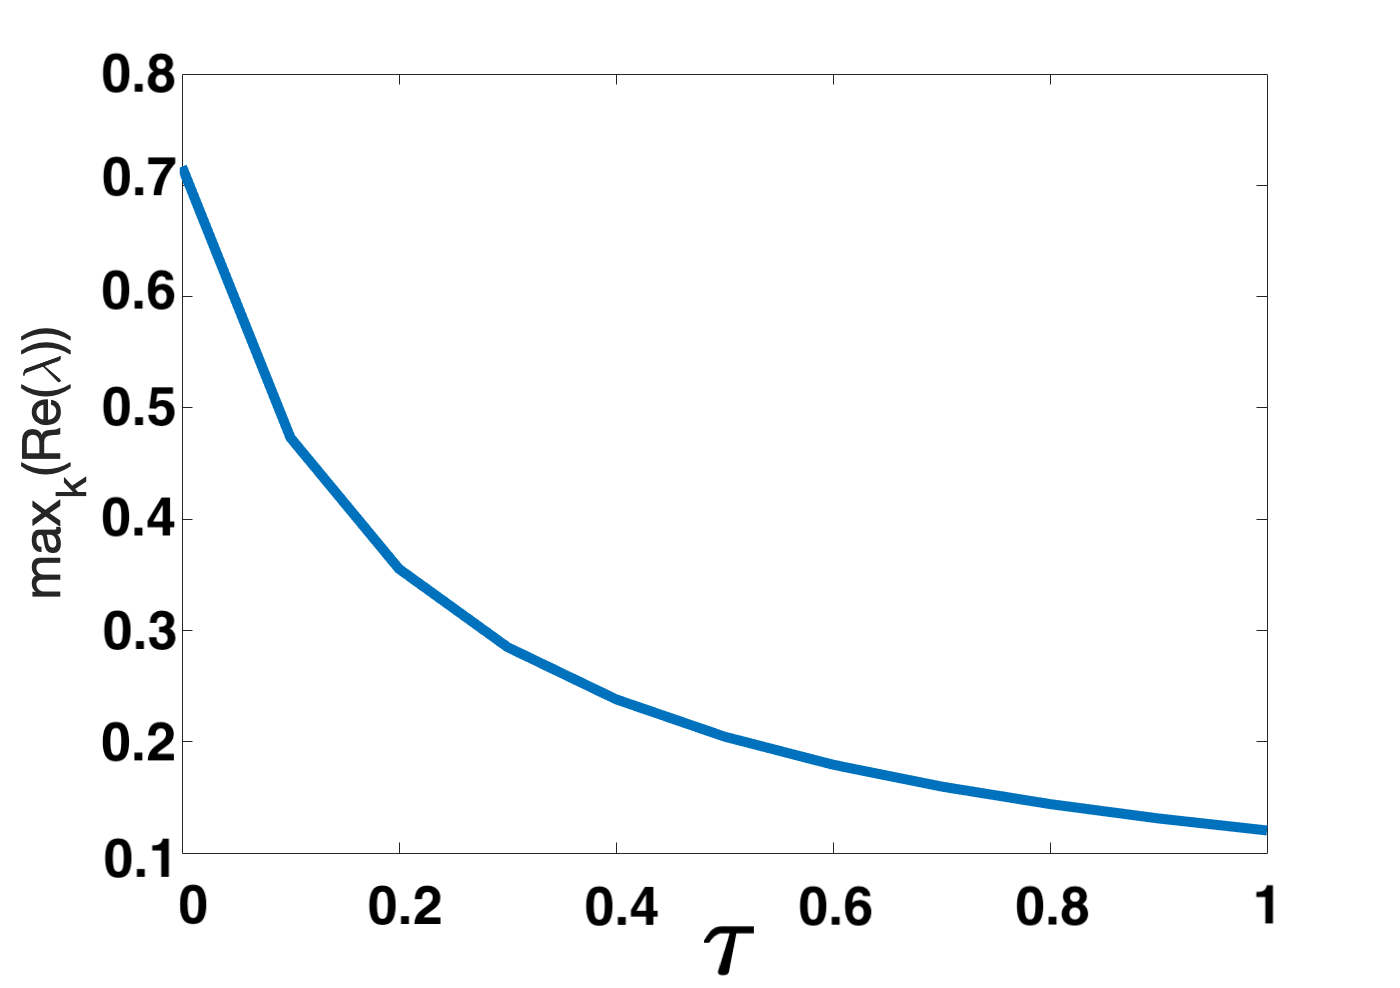
\includegraphics[width=8cm,height = 6cm]{disp2.png}
        \caption{$(a,b)=(0.1,0.9)$. $\max_k(\Re(\lambda))>0 \quad \forall\tau\in[0,1]$. Linear theory predicts pattern formation.}
        \label{}
    \end{subfigure}
    \caption{}
    \label{fig:dispfixed}
\end{figure}
Figure \ref{fig:dispfixed} suggests that for $(a,b)=(0.4,0.4)$ and $\tau\in[0,1]$, no patterns will form. However, we expect to see pattern formation $(a,b)=(0.1,0.9)$. We also hypothesise that since $\max_k(\Re(\lambda))$ at $\tau=0$ is greater than at $\tau=1$, the time taken to pattern formation will be longer at $\tau=1$. This relationship between time-to-pattern and time-delay is explored in more detail in section \ref{section:delaypatt}. Numerical results in figures \ref{fig:fixedsim1} and \ref{fig:fixedsim2} verify the findings from figure \ref{fig:dispfixed}, and suggest that the linear theory is a good approximation to the full model. We note by convention that the numerical solution of the activator $u$ is plotted.

\begin{figure}[H]
    \centering
    \begin{subfigure}[b]{0.45\textwidth}
        \centering
        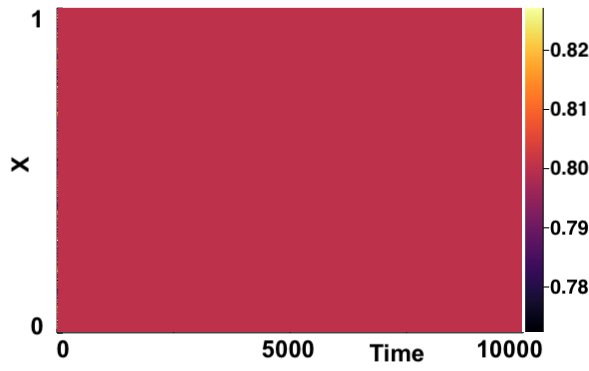
\includegraphics[width=8cm,height = 6cm]{nopatt1.png}
        \caption{$(a,b,\tau)=(0.4,0.4,0)$. No pattern formation after $t=10^4$. }
        \label{}
    \end{subfigure}
    \hfill
    \begin{subfigure}[b]{0.45\textwidth}
        \centering
        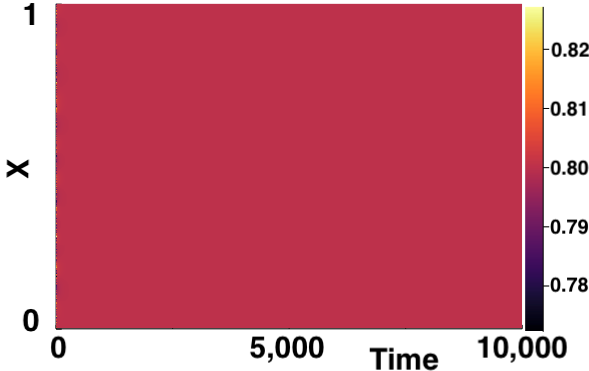
\includegraphics[width=8cm,height = 6cm]{nopatt2.png}
        \caption{$(a,b,\tau)=(0.4,0.4,1)$. No pattern formation after $t=10^4$.}
        \label{}
    \end{subfigure}
    \caption{}
    \label{fig:fixedsim1}
\end{figure}1

\begin{figure}[H]
    \centering
    \begin{subfigure}[b]{0.45\textwidth}
        \centering
        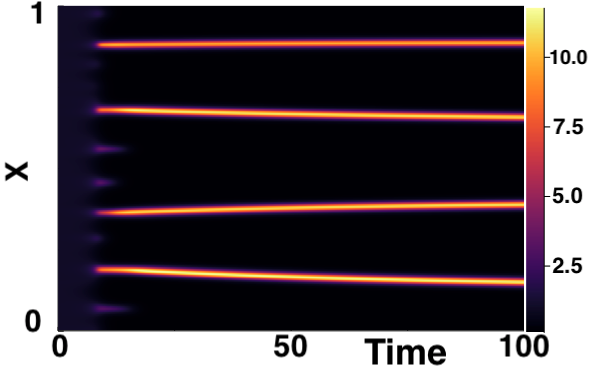
\includegraphics[width=8cm,height = 6cm]{patt1.png}
        \caption{$(a,b,\tau)=(0.1,0.9,0)$. Pattern formation at $t\approx7$ }
        \label{}
    \end{subfigure}
    \hfill
    \begin{subfigure}[b]{0.45\textwidth}
        \centering
        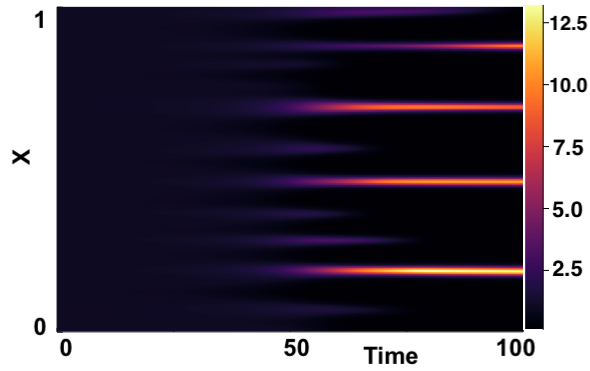
\includegraphics[width=8cm,height = 6cm]{patt2.png}
        \caption{$(a,b,\tau)=(0.1,0.9,1)$. Pattern formation at $t\approx50$.}
        \label{}
    \end{subfigure}
    \caption{}
    \label{fig:fixedsim2}
\end{figure}
These figures were produced using an initial condition $(u_0,v_0)$ given as a random Gaussian perturbation from the homogeneous steady-state. Namely, $$\begin{pmatrix}u_0\\v_0\end{pmatrix}=\begin{pmatrix}u_\star(1+r)\\v_\star(1+r)\end{pmatrix}$$ where $r$ is a random variable such that $r\sim\mathcal{N}(0,0.01)$. The notation $r\sim\mathcal{N}(\mu,\sigma^2)$ denotes a Normally distributed random variable $r$ with mean $\mu$ and standard deviation $\sigma$. A constant history function equal to the intitial conditions was used.
\subsection{Bifurcation Analysis}\label{section:fixedbif}
The Turing plot produced in figure \ref{fig:turingspace}, computed using the conditions in \eqref{cond1} and \eqref{cond2}, is a bifurcation diagram indication regions of Turing instability. We note two seperate curves which seperate the parameter space into it's distinct regions. These will be referred to as the `lines of stability'.
These two curves are indicated in figure \ref{fig:bif0}. The inner arc corresponds to the $(a,b)$ such that $\Re(\lambda)=0$ for the
spatially homogeneous characteristic equation $D_k$, namely when $k=0$. For $\tau=0$, this corresponds exactly to equating conditions $\eqref{cond1}$ to 0. The outer boundary is the points $(a,b)$ such that $\max_k\Re(\lambda)=0$ for the spatially inhomogeneous characteristic equation $D_k$. For $\tau=0$, this is exactly identical to equating to the conditions $\eqref{cond2}$ to 0.

By setting $\Re(\lambda)=0$ in equations \eqref{realfix} and \eqref{complexfix}, the real and imaginary parts of $D_k$ can be simplified to

\begin{align}\label{realfixbif}
  D_k^{\Re}&=-y^2\beta_k+[-\gamma_ky\sin(-y\tau)+\delta_k\cos(-y\tau)],\\
  D_k^{\text{Im}}&=\alpha_ky+[\gamma_ky\cos(-y\tau)+\delta_k\sin(-y\tau)].\label{complexfixbif}.
\end{align}


For a fixed $\tau$ and $b$, the roots of \eqref{realfixbif} and \eqref{complexfixbif} (at $k=0$) can be found for $a$ and $\text{Im}(\lambda)$.
Taking the $\max_k(a)$, a curve can be plotted in the $(a,b)$ parameter space for the outer boundary (and the inner arc) resulting in a bifurcation diagram of distinct regions where pattern formation will take place. We use a relatively large domain size of $\Omega=[0,30]$ and so the bifurcation diagram computed in this manner for $\tau=0$ should be a good approximation to the Turing space plot produced in figure \ref{fig:turingspace}. Figure \ref{fig:bif0} shows the bifurcation plot produced in this manner for $\tau=0$ along side the Turing space plot in figure \ref{fig:turingspace} for comparison.

\begin{figure}[H]
    \centering
    \begin{subfigure}[b]{0.47\textwidth}
        \centering
        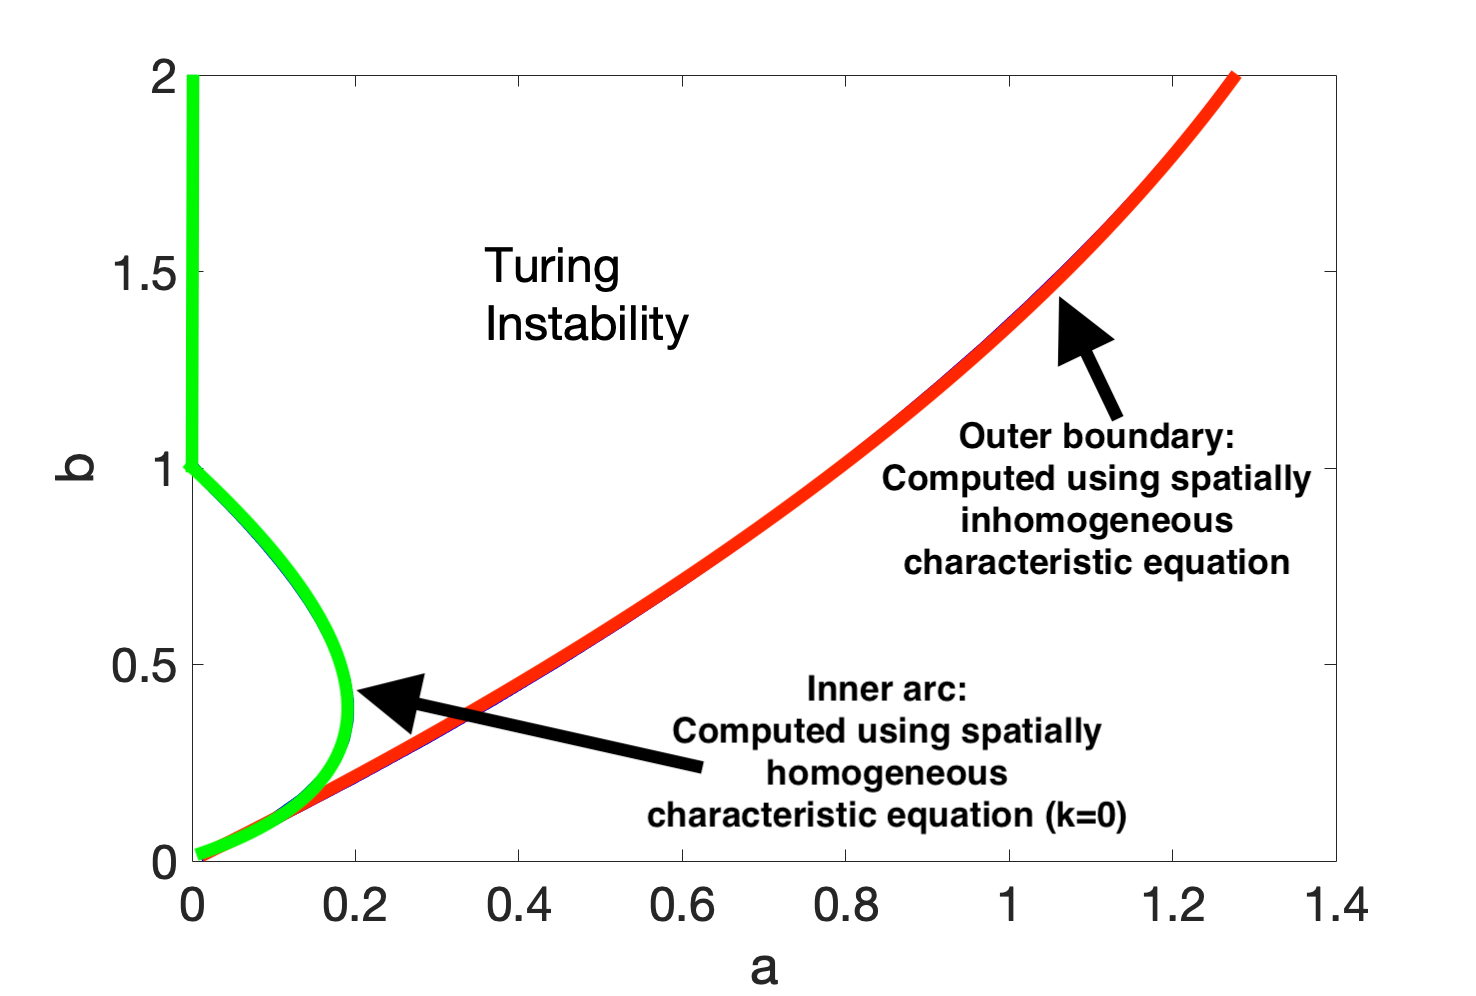
\includegraphics[width=9cm,height = 7cm]{bif0.png}
        \caption{Stability lines for $\tau=0$}
        \label{fig:bif0}
    \end{subfigure}
    \hfill
    \begin{subfigure}[b]{0.47\textwidth}
        \centering
        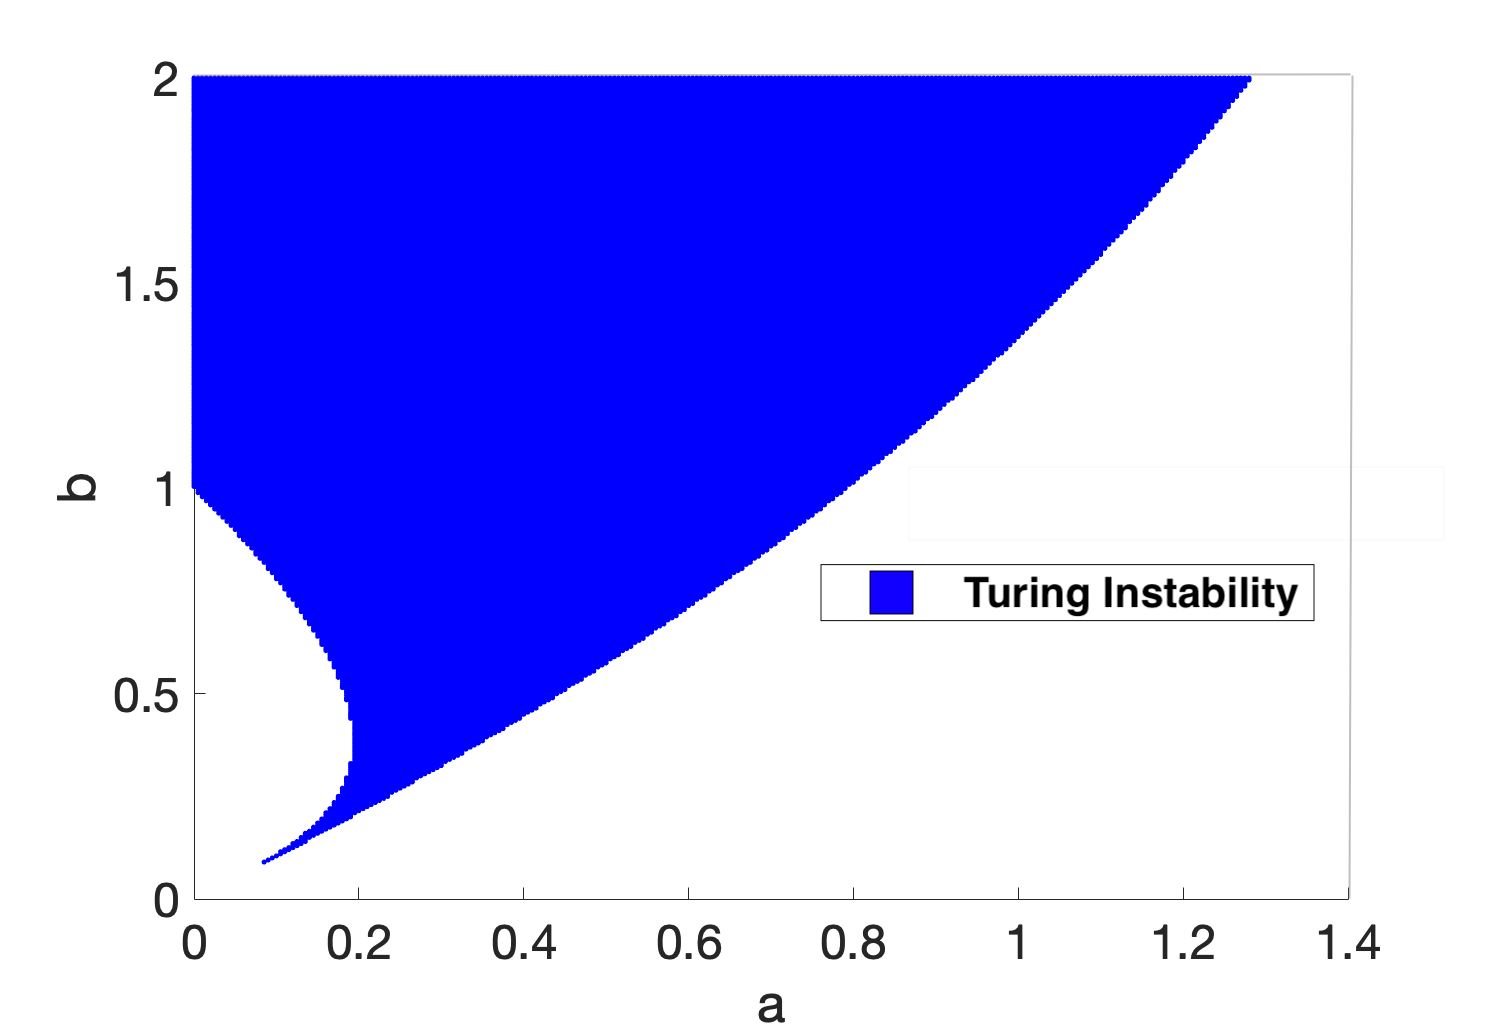
\includegraphics[width=9cm,height = 7cm]{turingspace.png}
        \caption{Turing space as in figure \ref{fig:turingspace}}
        \label{}
    \end{subfigure}
    \caption{}
    \label{fig:tspace1}
\end{figure}

Figure \ref{fig:tspacetau} shows the stability curves computed for a varying $\tau\in\{0,0.5,1,1.5\}$. It can be seen that, whilst the outer boundary computed from the characteristic equation for the spatially inhomgeneous model stays the same, the inner arc computed from using the characteristic equation from the spatially homogeneous model shifts to the left, increasing the region of parameter space for which Turing instabilities can occur. This observation matches results produced in \cite{william} for the spatially homogeneous LI model. This is also a similar result to that observed in \cite{fadai} for the Gierer-Meinhardt model. We see that for the LI model where delay-terms are placed solely in the activator dynamics, time-delay acts as a stabilising agent for pattern formation and increases the parameter space where pattern formation will occur.
\begin{figure}[H]
        \centering
        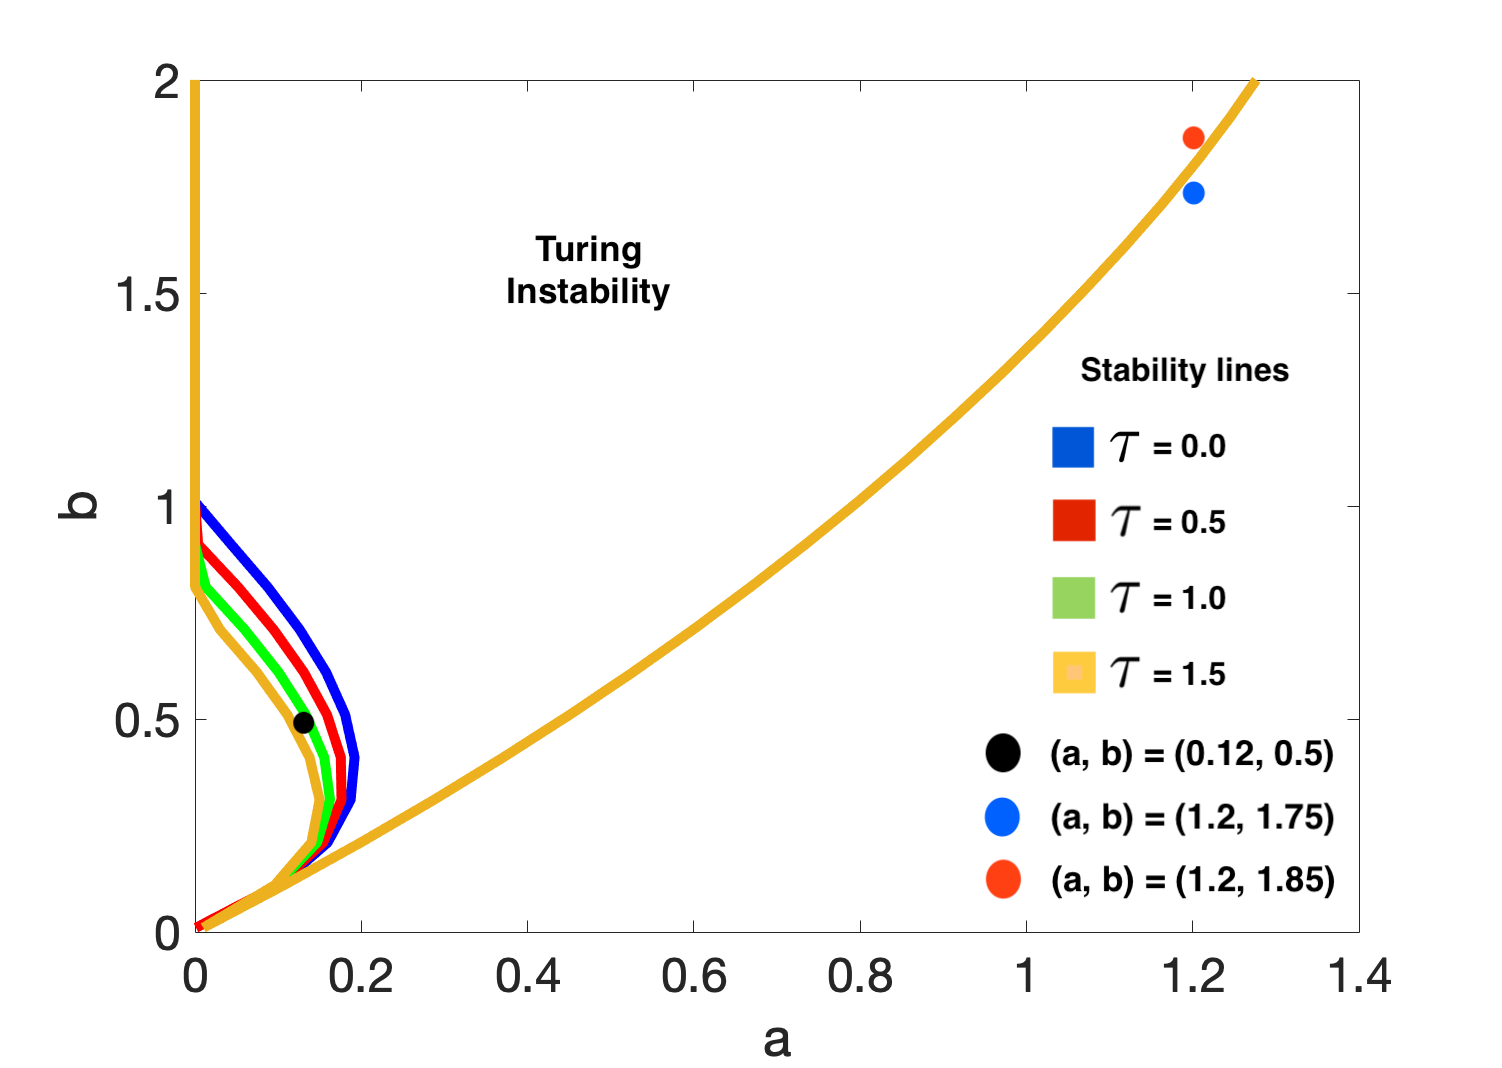
\includegraphics[width=12cm,height = 9cm]{tspacetau.png}
        \caption{Stability lines for $\tau\in\{0,0.5,1,1.5\}$}.
        \label{fig:tspacetau}
\end{figure}
We verify these results through numerical simulations. Three parameter points, $(a,b)=\{(0.12,0.5),(1.2,1.75),(1.2,1.85)\}$ are indicated in figure \ref{fig:tspacetau}. At $(a,b,\tau)=(0.12,0.5,0)$, linear theory suggests that there will be no pattern formation, but at $(a,b,\tau)=(0.12,0.5,1.5)$ there will be a Turing instability and thus patterns will form. Linear theory also suggests that for all $\tau\in\{0,0.5,1,1.5\}$, pattern formation will occur for $(a,b)=(1.2,1.85)$, but not for $(a,b)=(1.2,1.75)$. Numerical simulations for $(a,b)=(0.12,0.5)$ at $\tau=0,1.5$ are seen in figure \ref{fig:testturing}. Figures \ref{fig:testturing2} and \ref{fig:testturing3} show the results for numerical simulations at $(a,b)=\{(1.2,1.75),(1.2,1.85)\}$ for $\tau=\{0,0.5,1,1.5\}$.
\begin{figure}[h]
    \centering
    \begin{subfigure}[b]{0.45\textwidth}
        \centering
        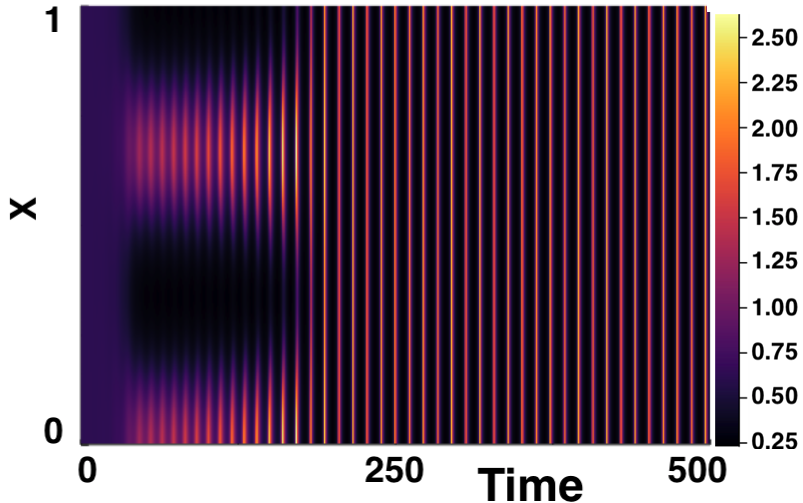
\includegraphics[width=7cm,height=5cm]{toscill.png}
        \caption{$\tau=0$. Oscillations seen.}
        \label{}
    \end{subfigure}
    \hfill
    \begin{subfigure}[b]{0.45\textwidth}
        \centering
        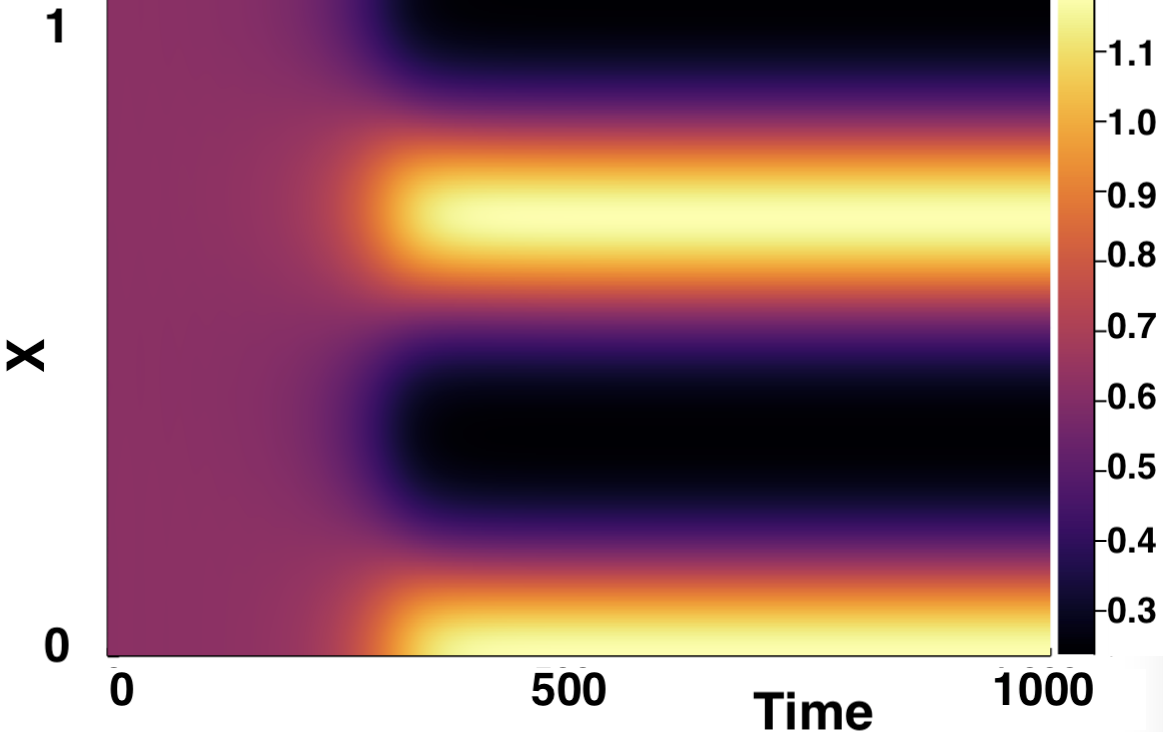
\includegraphics[width=7cm,height=5cm]{tpattpred.png}
        \caption{$\tau=1.5$. Pattern formation seen.}
        \label{}
    \end{subfigure}
    \caption{Numerical simulations produced with parameters $(a,b,\epsilon^2)=(0.12,0.5,0.1)$, for $\tau=0,1.5$. Linear theory suggests we seen pattern formation at $\tau=1.5$ but not at $\tau=0$.}
    \label{fig:testturing}
\end{figure}

\begin{figure}[h]
    \centering
    \begin{subfigure}[b]{0.45\textwidth}
        \centering
        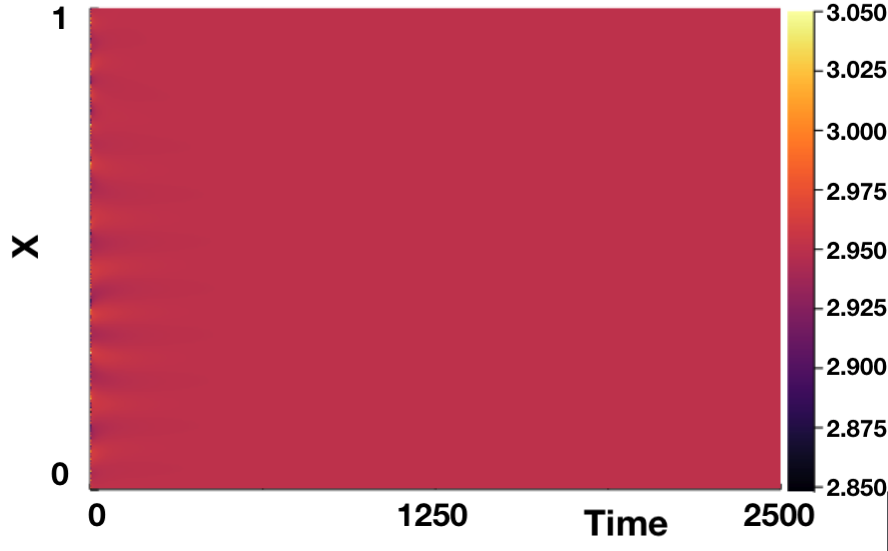
\includegraphics[width=7cm,height=5cm]{p3t0.png}
        \caption{$\tau=0$.}
        \label{}
    \end{subfigure}
    \hfill
    \begin{subfigure}[b]{0.45\textwidth}
        \centering
        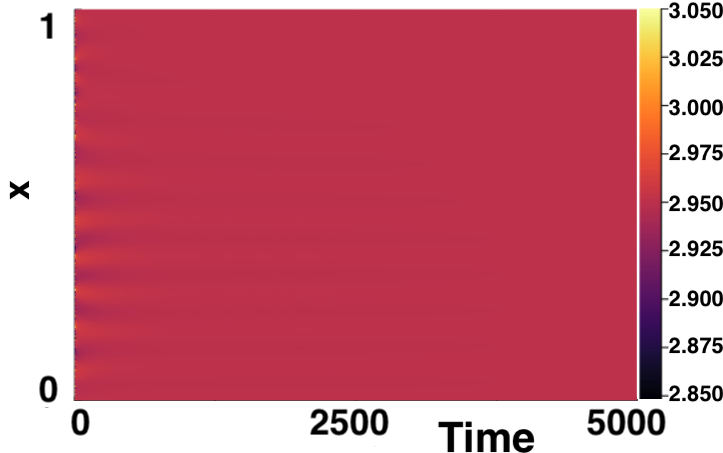
\includegraphics[width=7cm,height=5cm]{p3t05.png}
        \caption{$\tau=0.5$}
        \label{}
    \end{subfigure}
    \hfill
    \begin{subfigure}[b]{0.45\textwidth}
        \centering
        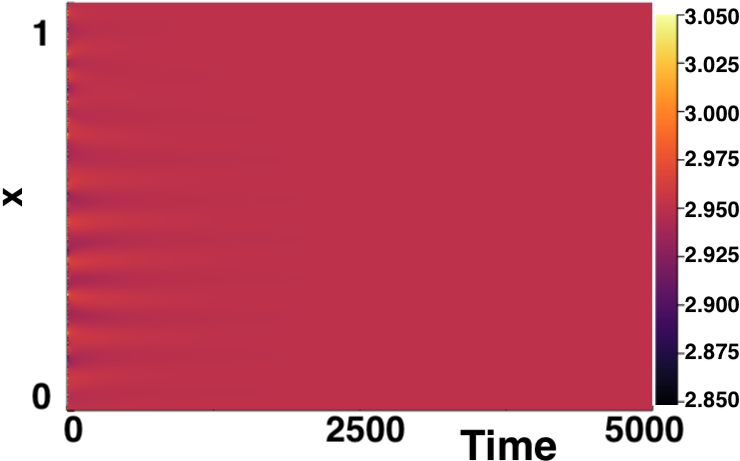
\includegraphics[width=7cm,height=5cm]{p3t1.png}
        \caption{$\tau=1$}
        \label{}
    \end{subfigure}
    \hfill
    \begin{subfigure}[b]{0.45\textwidth}
        \centering
        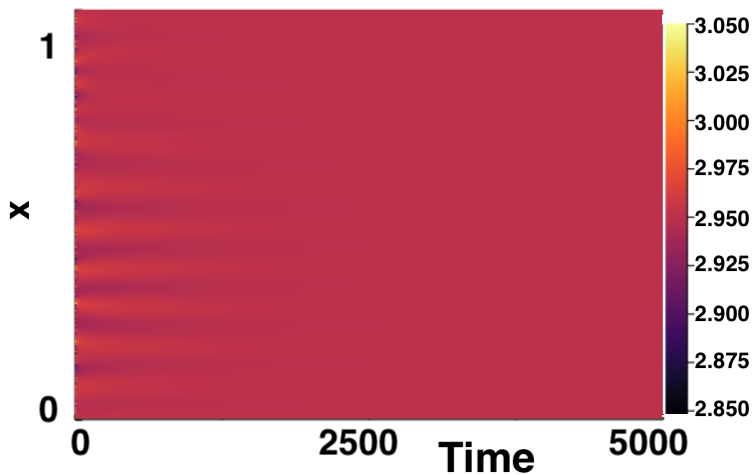
\includegraphics[width=7cm,height=5cm]{p3t15.png}
        \caption{$\tau=1.5$.}
        \label{}
    \end{subfigure}
    \caption{Numerical simulations for $(a,b)=(1.2,1.75)$. We see no pattern formation for $\tau\in\{0,0.5,1,1.5\}$ as suggested by linear theory.}
    \label{fig:testturing2}
\end{figure}

\begin{figure}[H]
    \centering
    \begin{subfigure}[b]{0.45\textwidth}
        \centering
        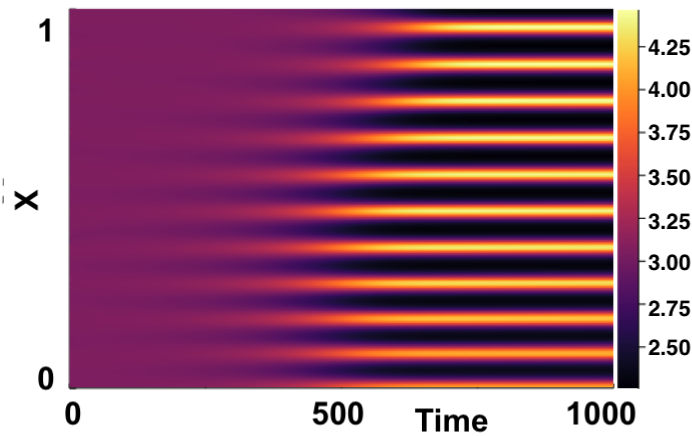
\includegraphics[width=7cm,height=5cm]{p2t0.png}
        \caption{$\tau=0$.}
        \label{}
    \end{subfigure}
    \hfill
    \begin{subfigure}[b]{0.45\textwidth}
        \centering
        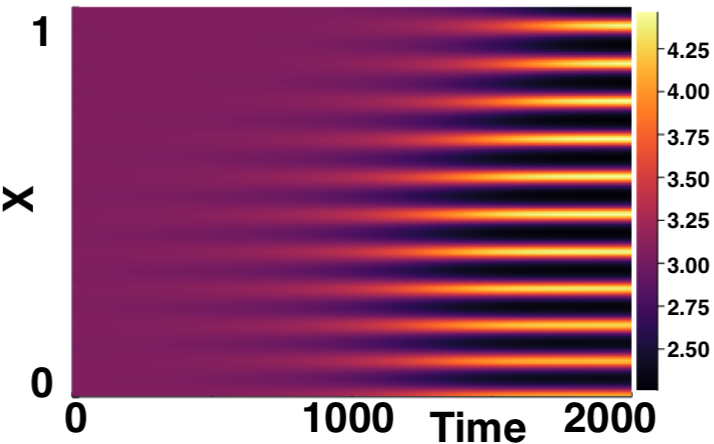
\includegraphics[width=7cm,height=5cm]{p2t05.png}
        \caption{$\tau=0.5$}
        \label{}
    \end{subfigure}
    \hfill
    \begin{subfigure}[b]{0.45\textwidth}
        \centering
        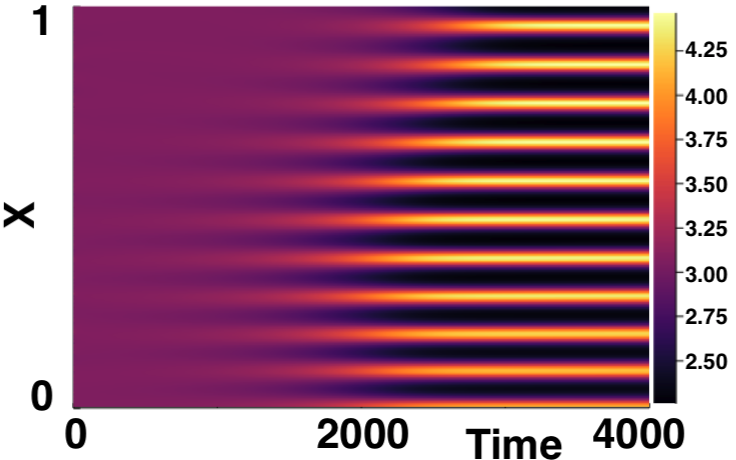
\includegraphics[width=7cm,height=5cm]{p2t1.png}
        \caption{$\tau=1$}
        \label{}
    \end{subfigure}
    \hfill
    \begin{subfigure}[b]{0.45\textwidth}
        \centering
        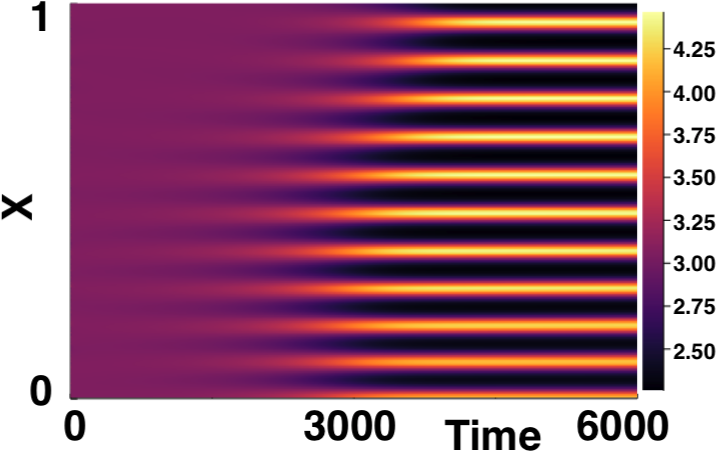
\includegraphics[width=7cm,height=5cm]{p2t15.png}
        \caption{$\tau=1.5$.}
        \label{}
    \end{subfigure}
    \caption{Numerical simulations for $(a,b)=(1.2,1.85)$. We see pattern formation on an increasing time-scale for $\tau\in\{0,0.5,1,1.5\}$ as suggested by linear theory.}
    \label{fig:testturing3}
\end{figure}

Figure \ref{fig:tspacetau} shows how the time-delay affects the region of Turing instability, but it provides no information as to how $\max_k(\Re(\lambda_k))$ varies as $\tau$ increases over the $(a,b)$ parameter space. In figure \ref{fig:lambdavary} we plot a heatmap of $\max_k(\Re(\lambda_k))$ over the $(a,b)$ parameter space for vay
rying $\tau\in\{0,0.5,1,1.5\}$. Overlayed onto these plots are contour lines corresponding to where $\Re(\lambda_0)=0$ and $\max_k(\Re(\lambda_k))=0$, highlighting the Turing instability region. The plots were produced with $\epsilon^2=0.001$ and a domain $\Omega=[0,30]$, with $\max_k$ taken over $k\in[0,20]$ at regular discrete intervals of $1$.
\begin{figure}[H]
    \centering
    \begin{subfigure}[b]{0.45\textwidth}
        \centering
        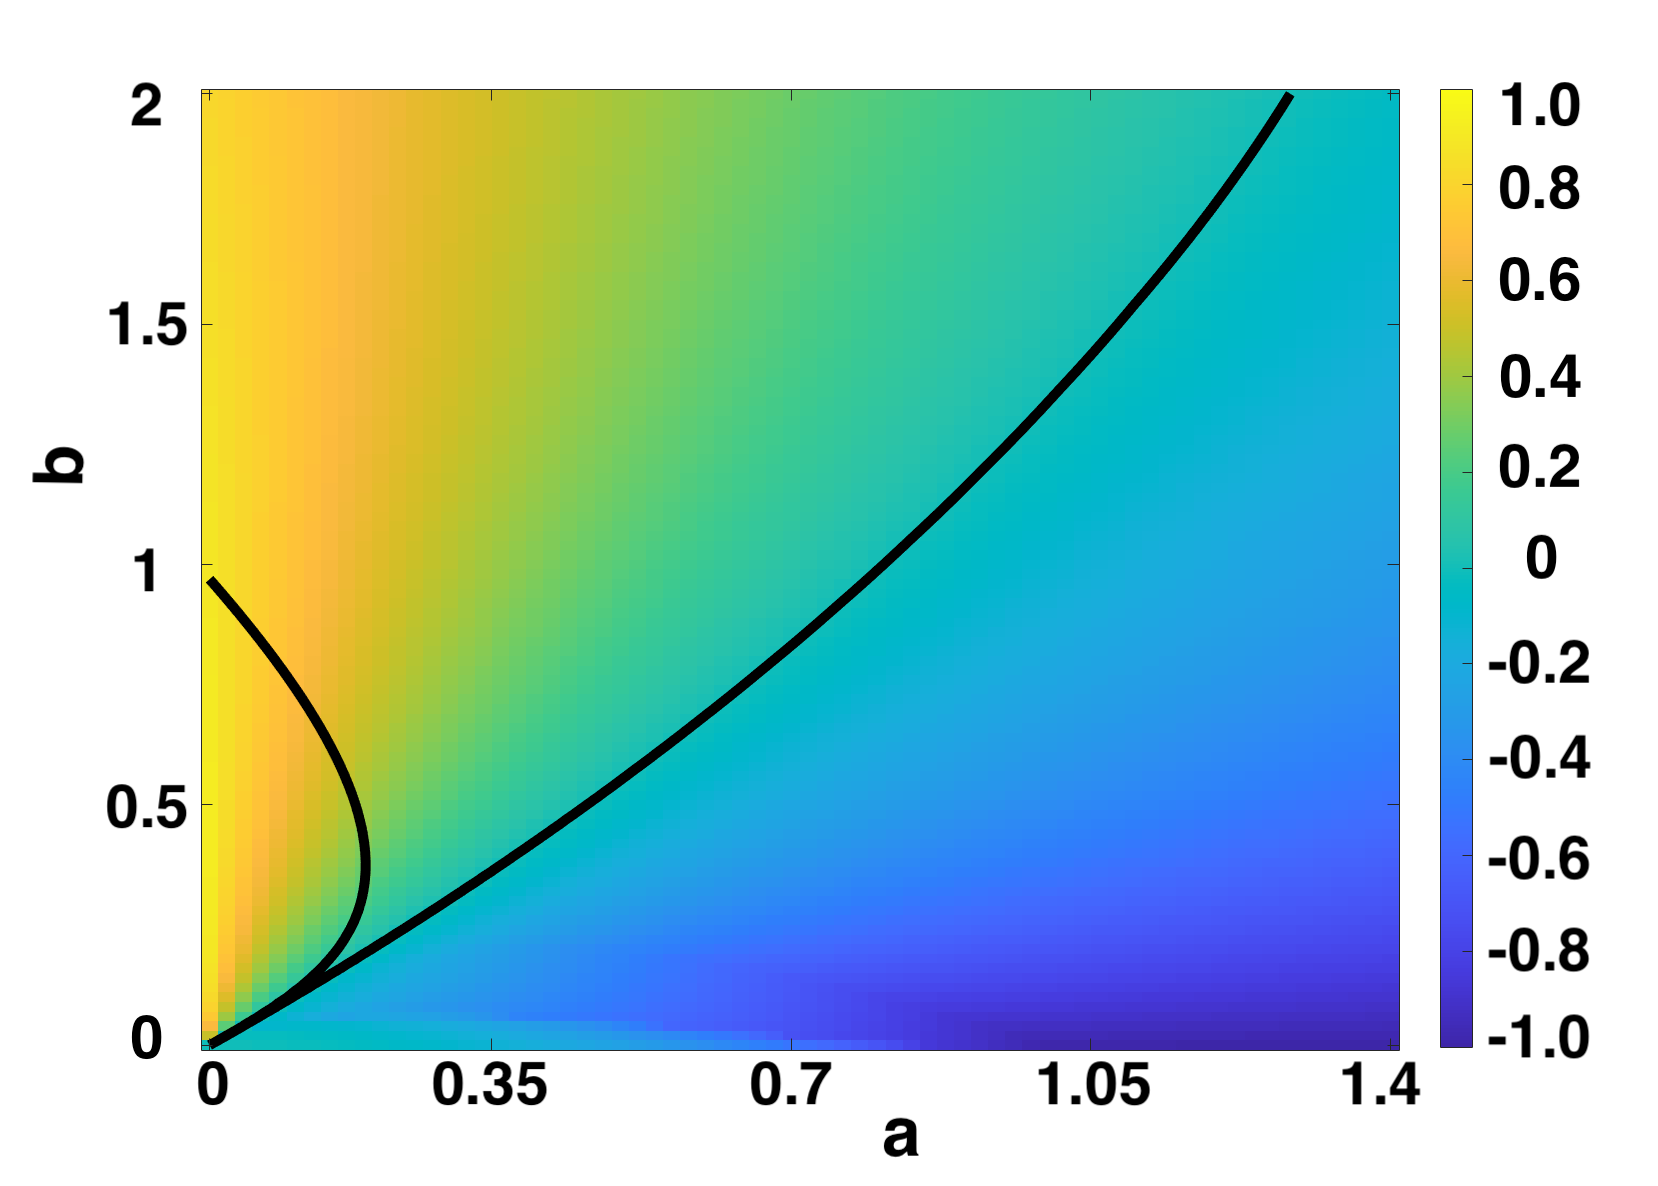
\includegraphics[width=7cm,height=5cm]{tau0bif.png}
        \caption{$\tau=0$.}
        \label{}
    \end{subfigure}
    \hfill
    \begin{subfigure}[b]{0.45\textwidth}
        \centering
        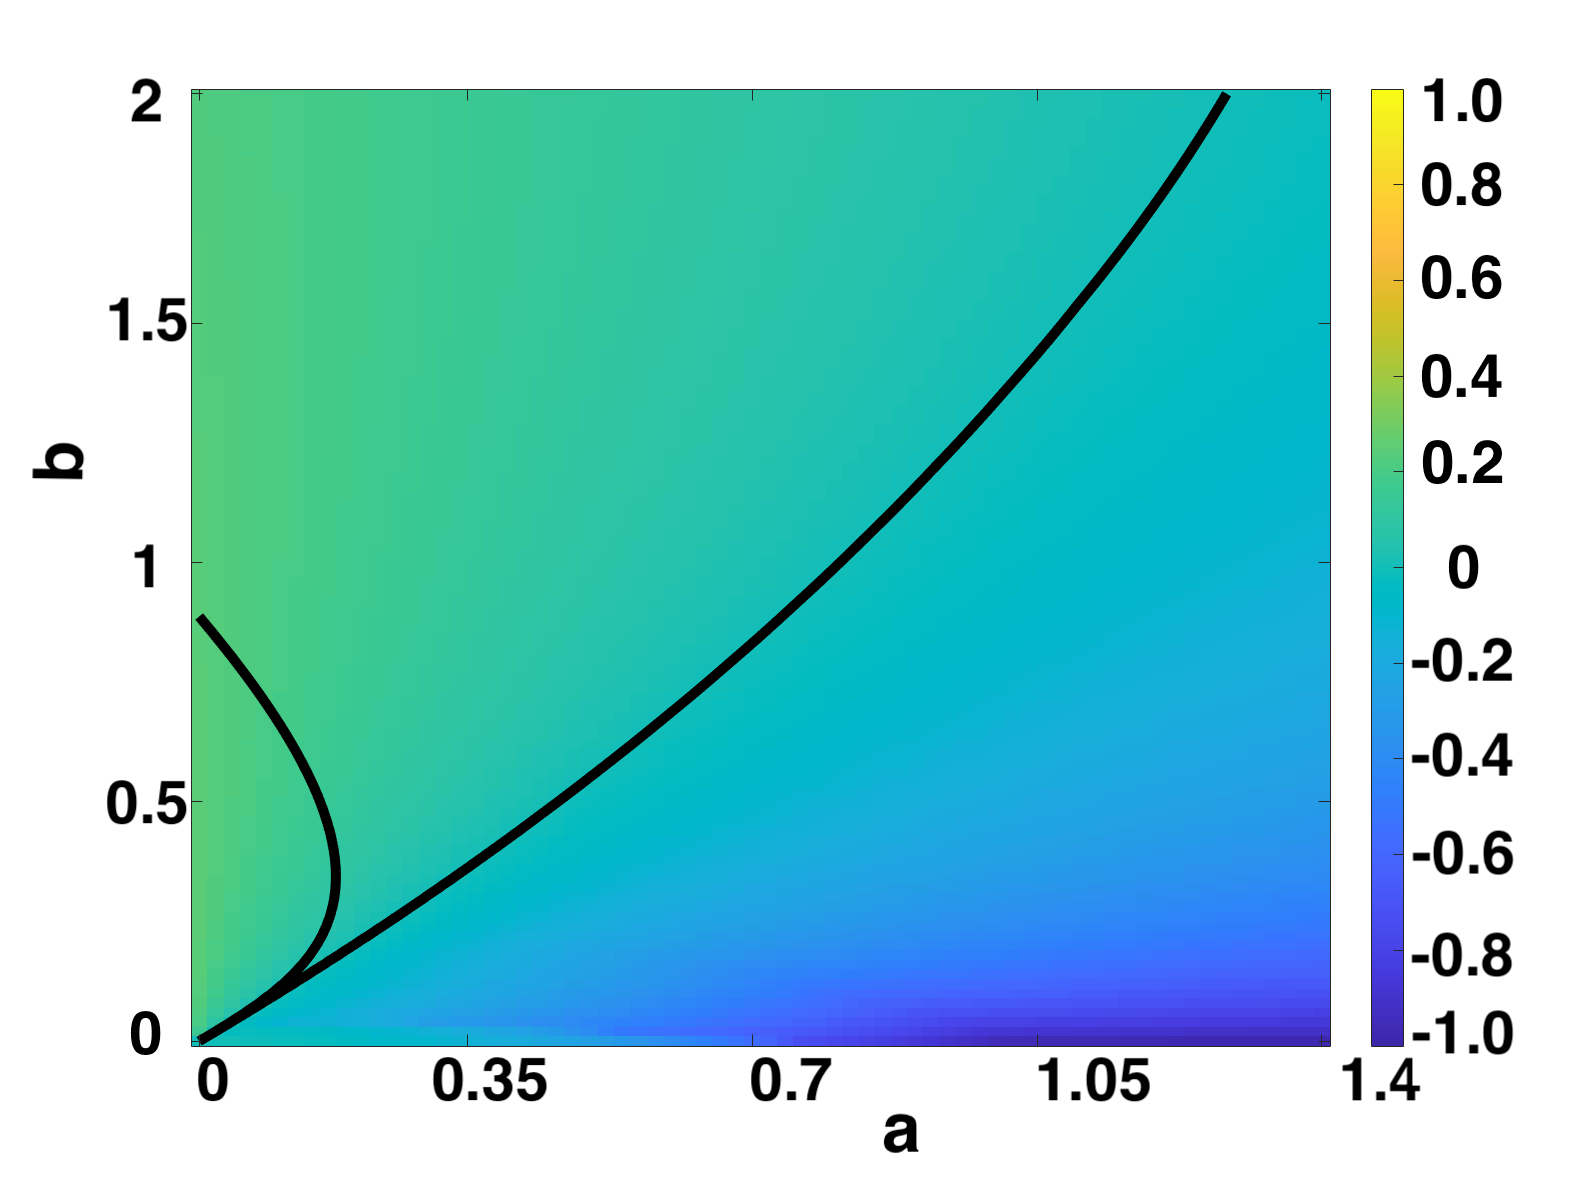
\includegraphics[width=7cm,height=5cm]{tau05bif.png}
        \caption{$\tau=0.5$}
        \label{}
    \end{subfigure}
    \hfill
    \begin{subfigure}[b]{0.45\textwidth}
        \centering
        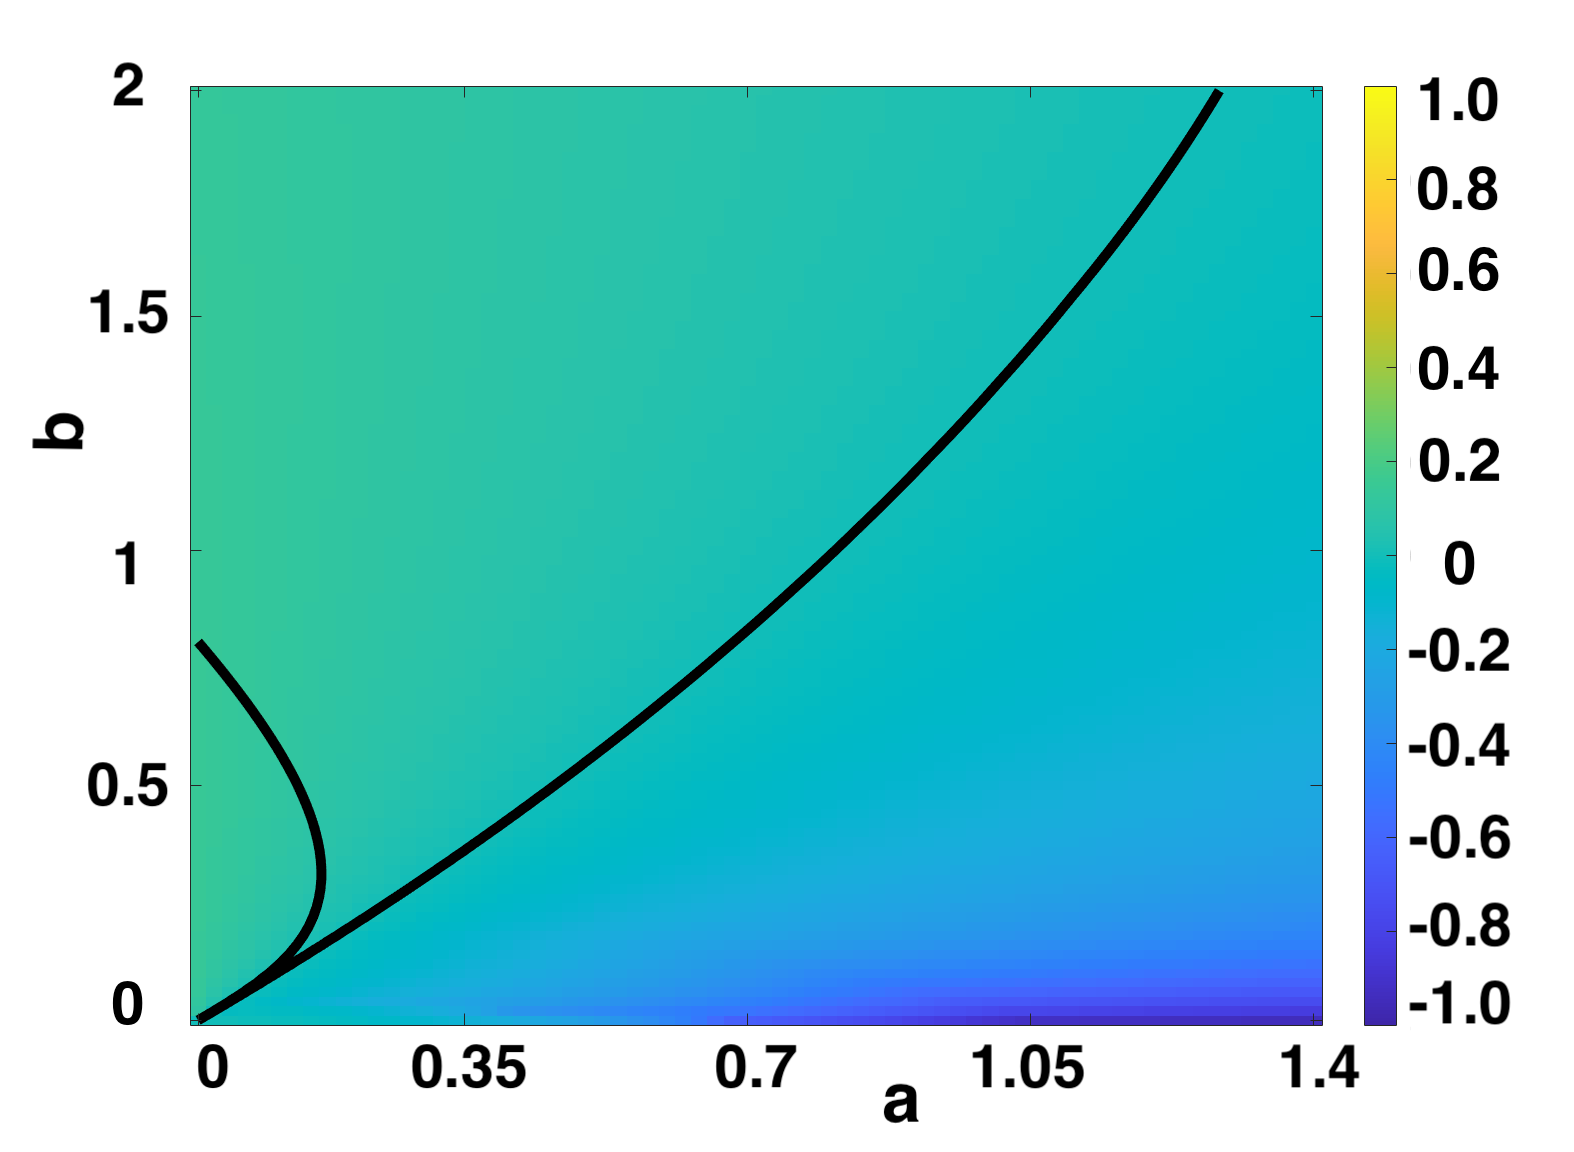
\includegraphics[width=7cm,height=5cm]{tau1bif.png}
        \caption{$\tau=1$}
        \label{}
    \end{subfigure}
    \hfill
    \begin{subfigure}[b]{0.45\textwidth}
        \centering
        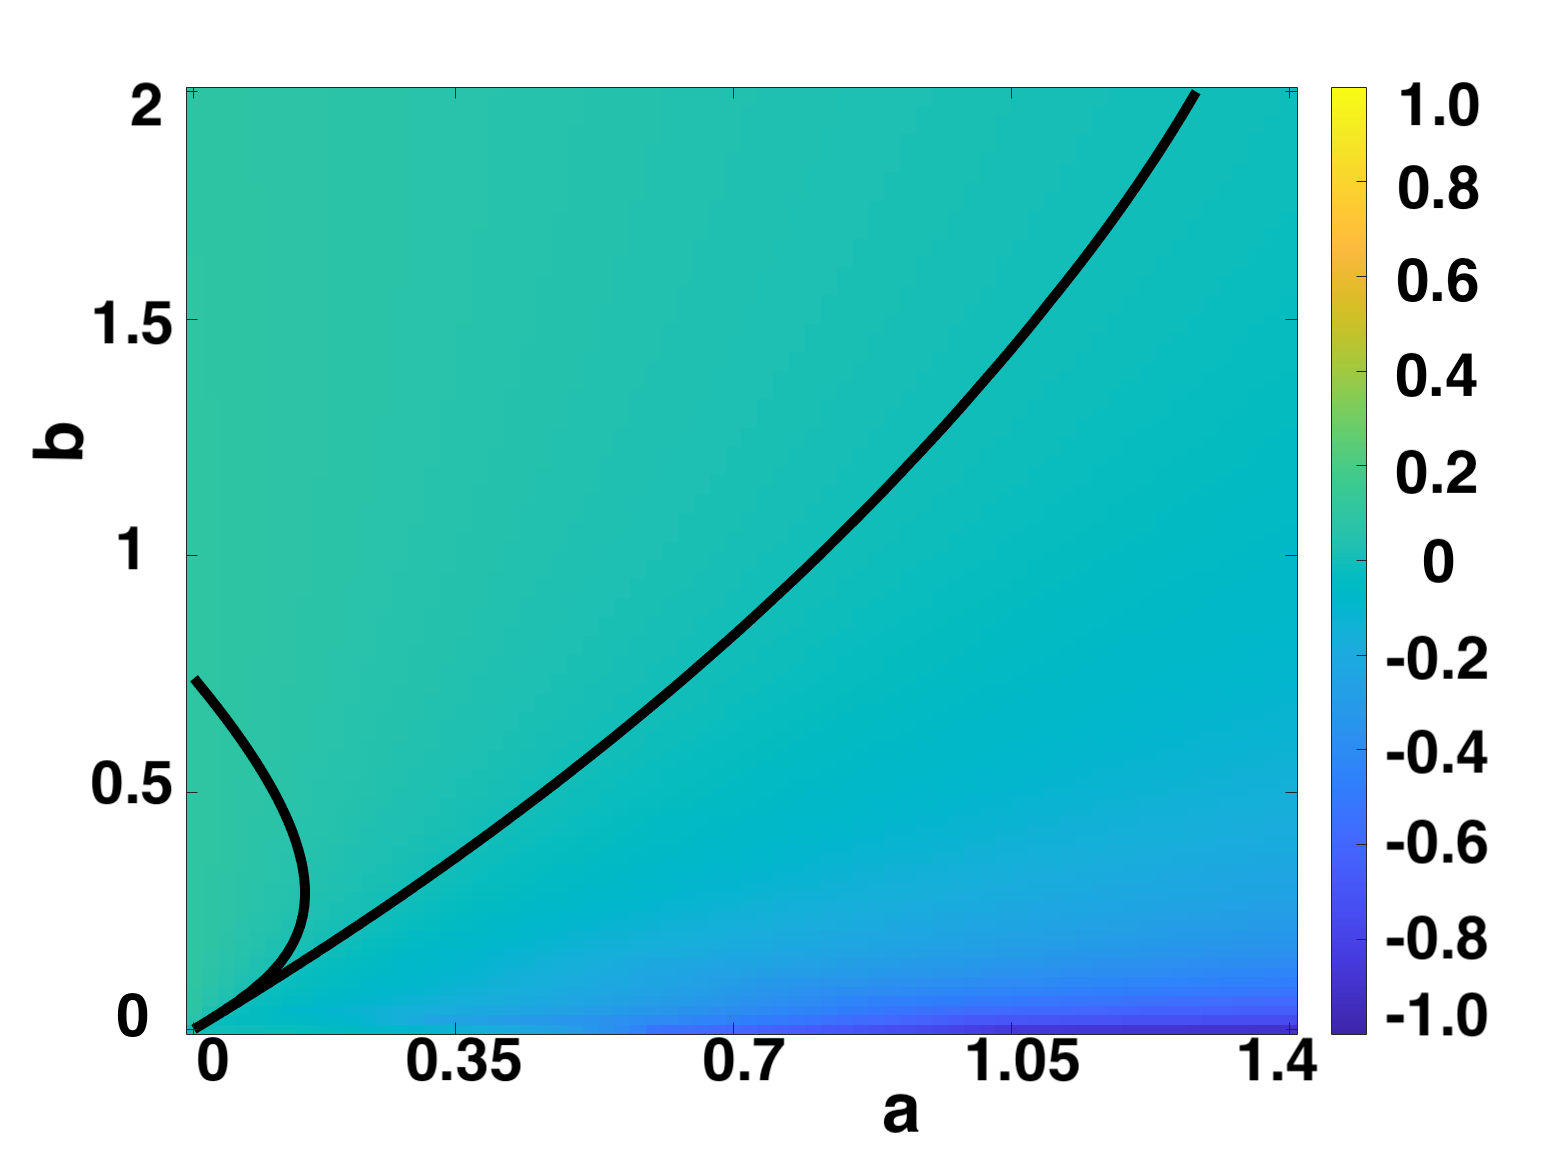
\includegraphics[width=7cm,height=5cm]{tau15bif.png}
        \caption{$\tau=1.5$.}
        \label{}
    \end{subfigure}
    \caption{$\max_k(\Re(\lambda_k))$ computed over $(a,b)$ parameter space, with $\epsilon^2=0.001$. As $\tau$ increases, $|\max_k(\Re(\lambda_k))|$ decreases.}
    \label{fig:lambdavary}
\end{figure}
As $\tau$ increases, it can be seen that the absolute value $|\max_k(\Re((\lambda_k)))|$. This suggests that for $(a,b)$ values within the Turing instability region, pattern formation will take longer to occur. It also suggests however that for $(a,b)$ such that $\max_k(\Re(\lambda_k))<0$, it will take a longer time for the eigenfunctions with modes $k\neq0$ to decay to a spatially homogeneous steady-state. We see this behaviour in figure \ref{fig:decaytime}, where numerical solutions are shown on a time-span of $[0,10]$ for $(a,b)=(1.2,0.1)$ with varying $\tau\in\{0,0.5,1,1.5\}$. It can be seen that the time-taken for the initial perturbation to fully decay back to a spatially homogeneous steady-state increases as $\tau$ increases. A black vertical line has been appended onto the plots to indicate
\begin{figure}[H]
    \centering
    \begin{subfigure}[b]{0.45\textwidth}
        \centering
        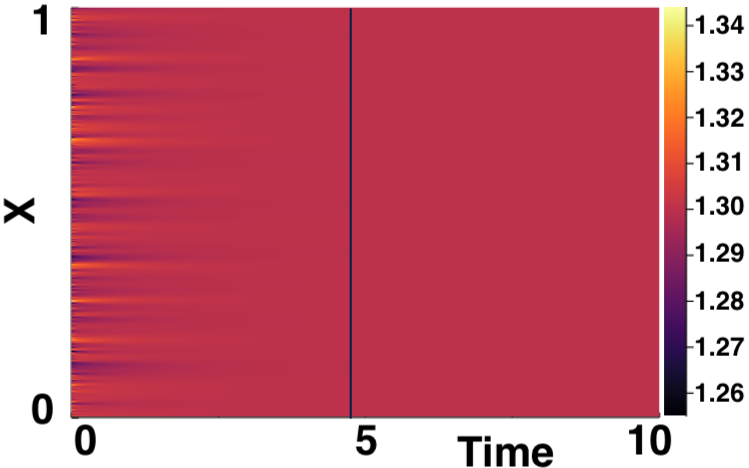
\includegraphics[width=8cm,height=6cm]{decay1.png}
        \caption{$\tau=0$.}
        \label{}
    \end{subfigure}
    \hfill
    \begin{subfigure}[b]{0.45\textwidth}
        \centering
        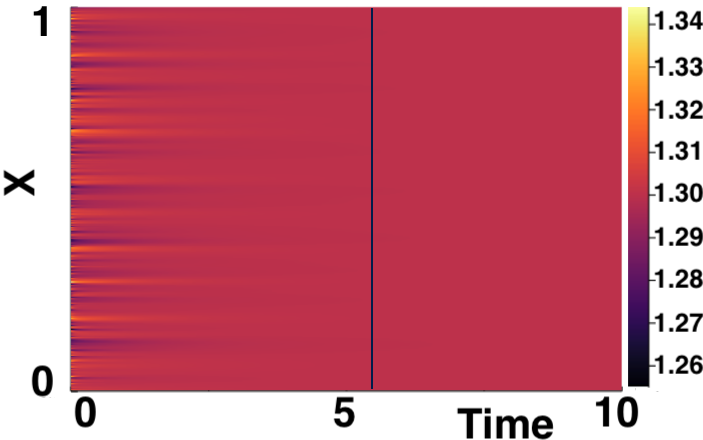
\includegraphics[width=8cm,height=6cm]{decay2.png}
        \caption{$\tau=0.5$}
        \label{}
    \end{subfigure}
    \hfill
    \begin{subfigure}[b]{0.45\textwidth}
        \centering
        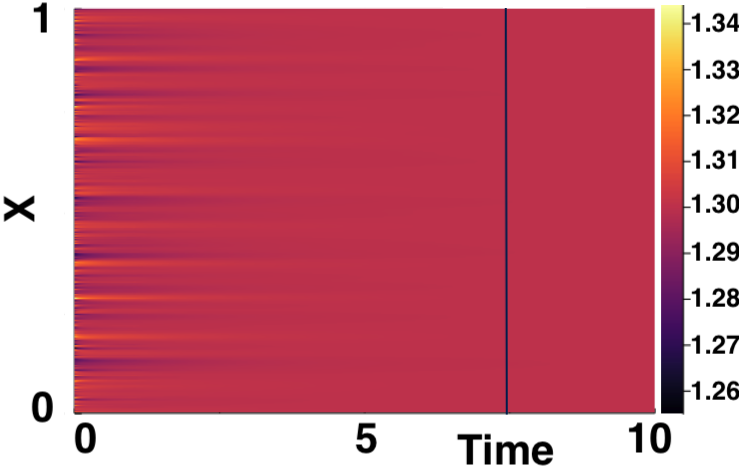
\includegraphics[width=8cm,height=6cm]{decay3.png}
        \caption{$\tau=1$}
        \label{}
    \end{subfigure}
    \hfill
    \begin{subfigure}[b]{0.45\textwidth}
        \centering
        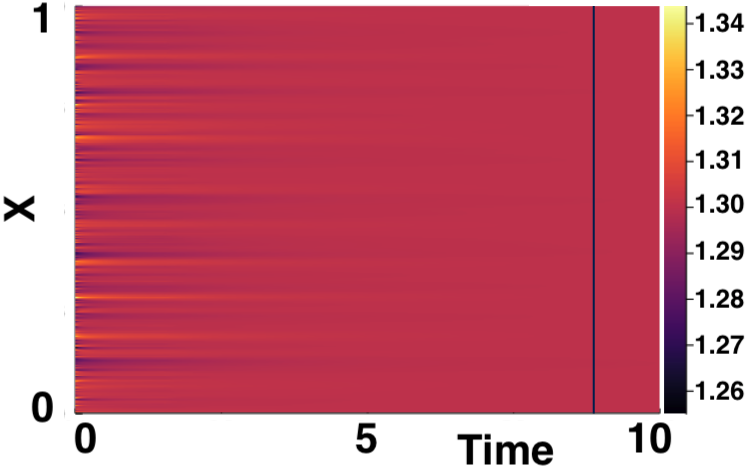
\includegraphics[width=8cm,height=6cm]{decay4.png}
        \caption{$\tau=1.5$.}
        \label{}
    \end{subfigure}
    \caption{Numerical simulations for $(a,b)=(1.2,0.1)$ at varying $\tau\in\{0,0.5,1,1.5\}$. As $\tau$ increases, the length of time until the perturbation decays to a spatially homogeneous steady-state also increases.}
    \label{fig:decaytime}
\end{figure}
Figure \ref{fig:fixbif2} shows analogous bifurcation diagrams as in figure \ref{fig:lambdavary}, but with $\epsilon^2=0.1$. We note that as the ratio, $\epsilon^2$, of diffusion constants in the reaction-diffusion constant moves closer to $1$, the region of parameter space exhibiting Turing instability decreases. It can be observed however that altering $\epsilon^2$ does not change the effect that an increasing $\tau$ has on $\max_k(\Re(\lambda_k))$, and that increasing the delay $\tau$ continues to act as a stabilising agent for Turing instabilities, with a shifting of the spatially homogeneous inner arc.

\begin{figure}[H]
    \centering
    \begin{subfigure}[b]{0.45\textwidth}
        \centering
        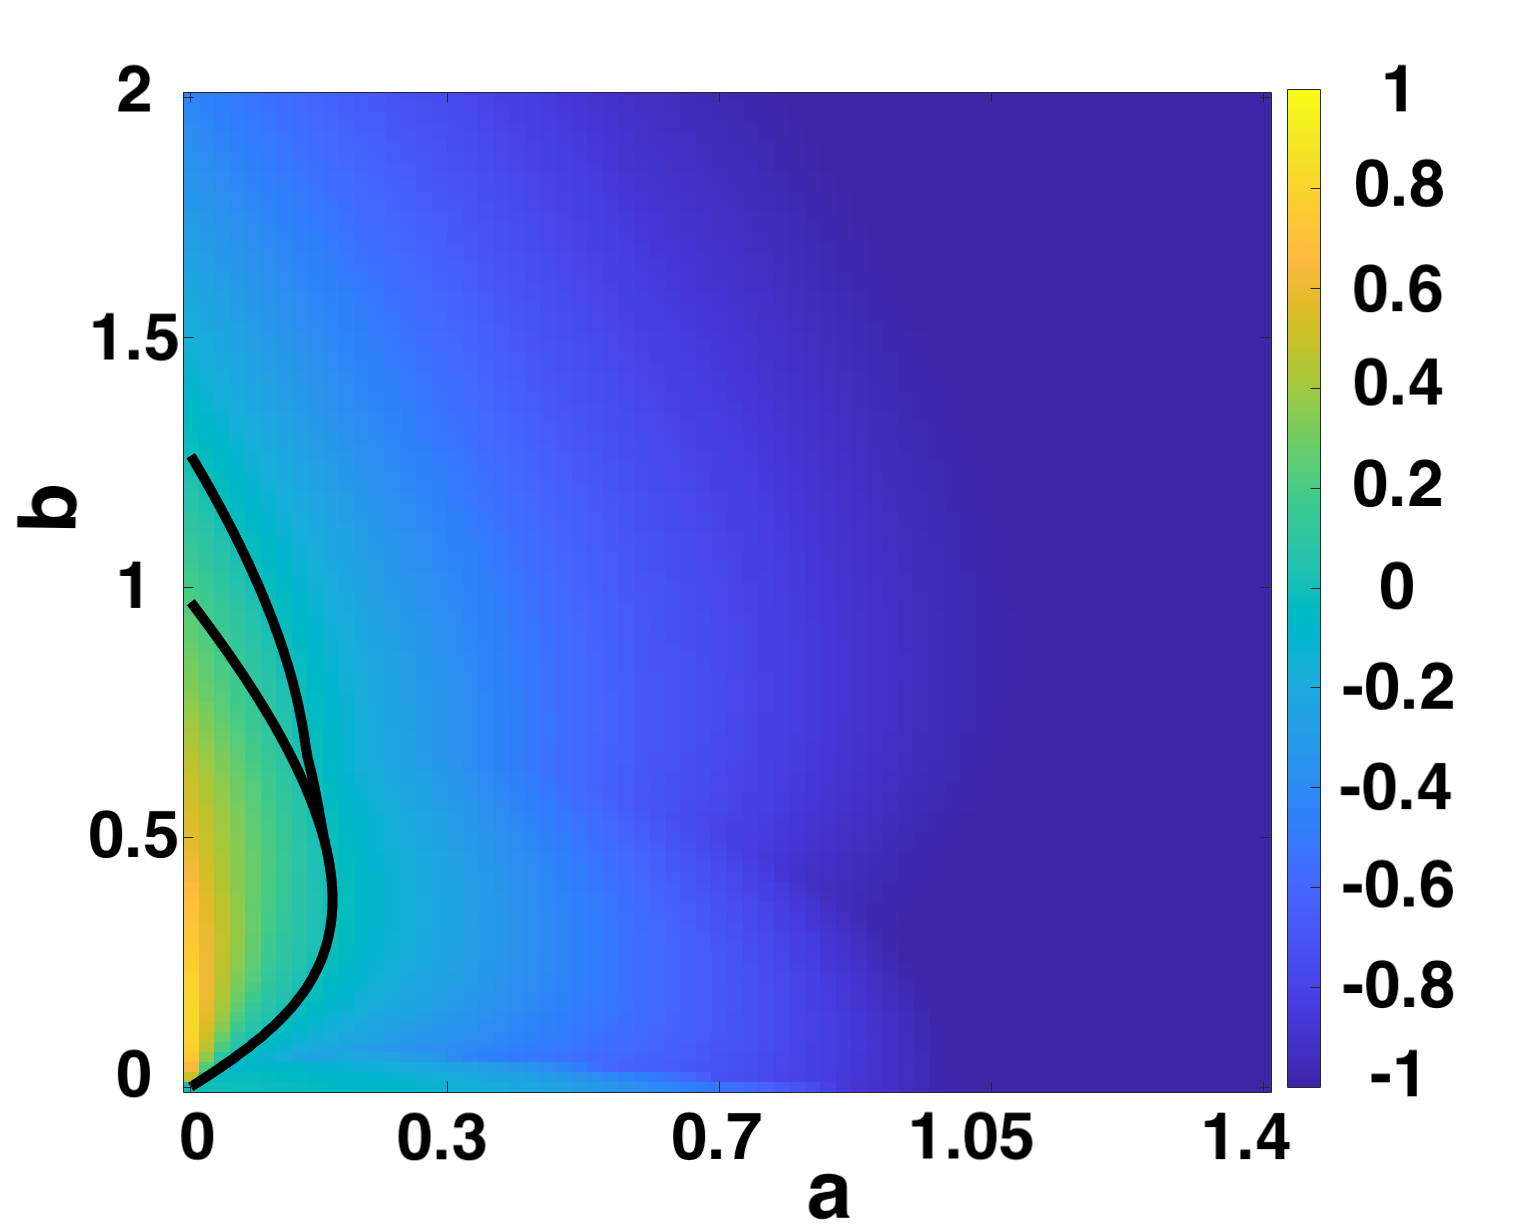
\includegraphics[width=7cm,height=5cm]{fixbif21.png}
        \caption{$\tau=0$.}
        \label{}
    \end{subfigure}
    \hfill
    \begin{subfigure}[b]{0.45\textwidth}
        \centering
        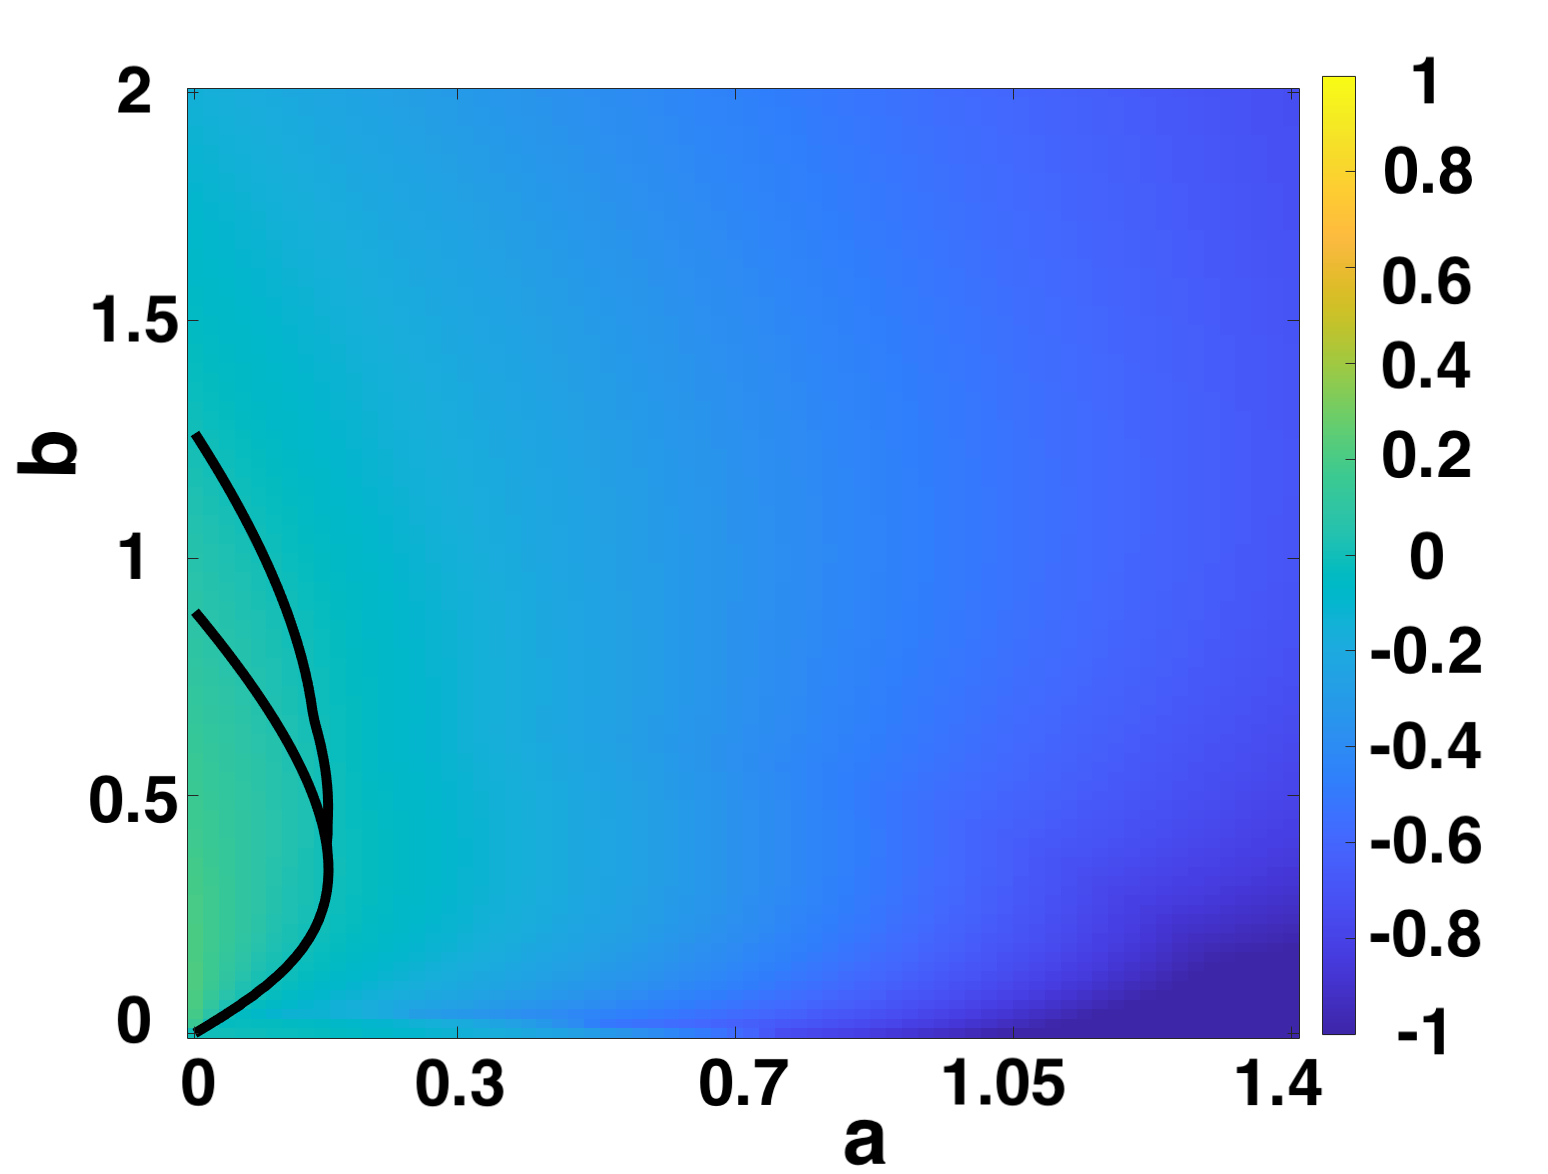
\includegraphics[width=7cm,height=5cm]{fixbif22.png}
        \caption{$\tau=0.5$}
        \label{}
    \end{subfigure}
    \hfill
    \begin{subfigure}[b]{0.45\textwidth}
        \centering
        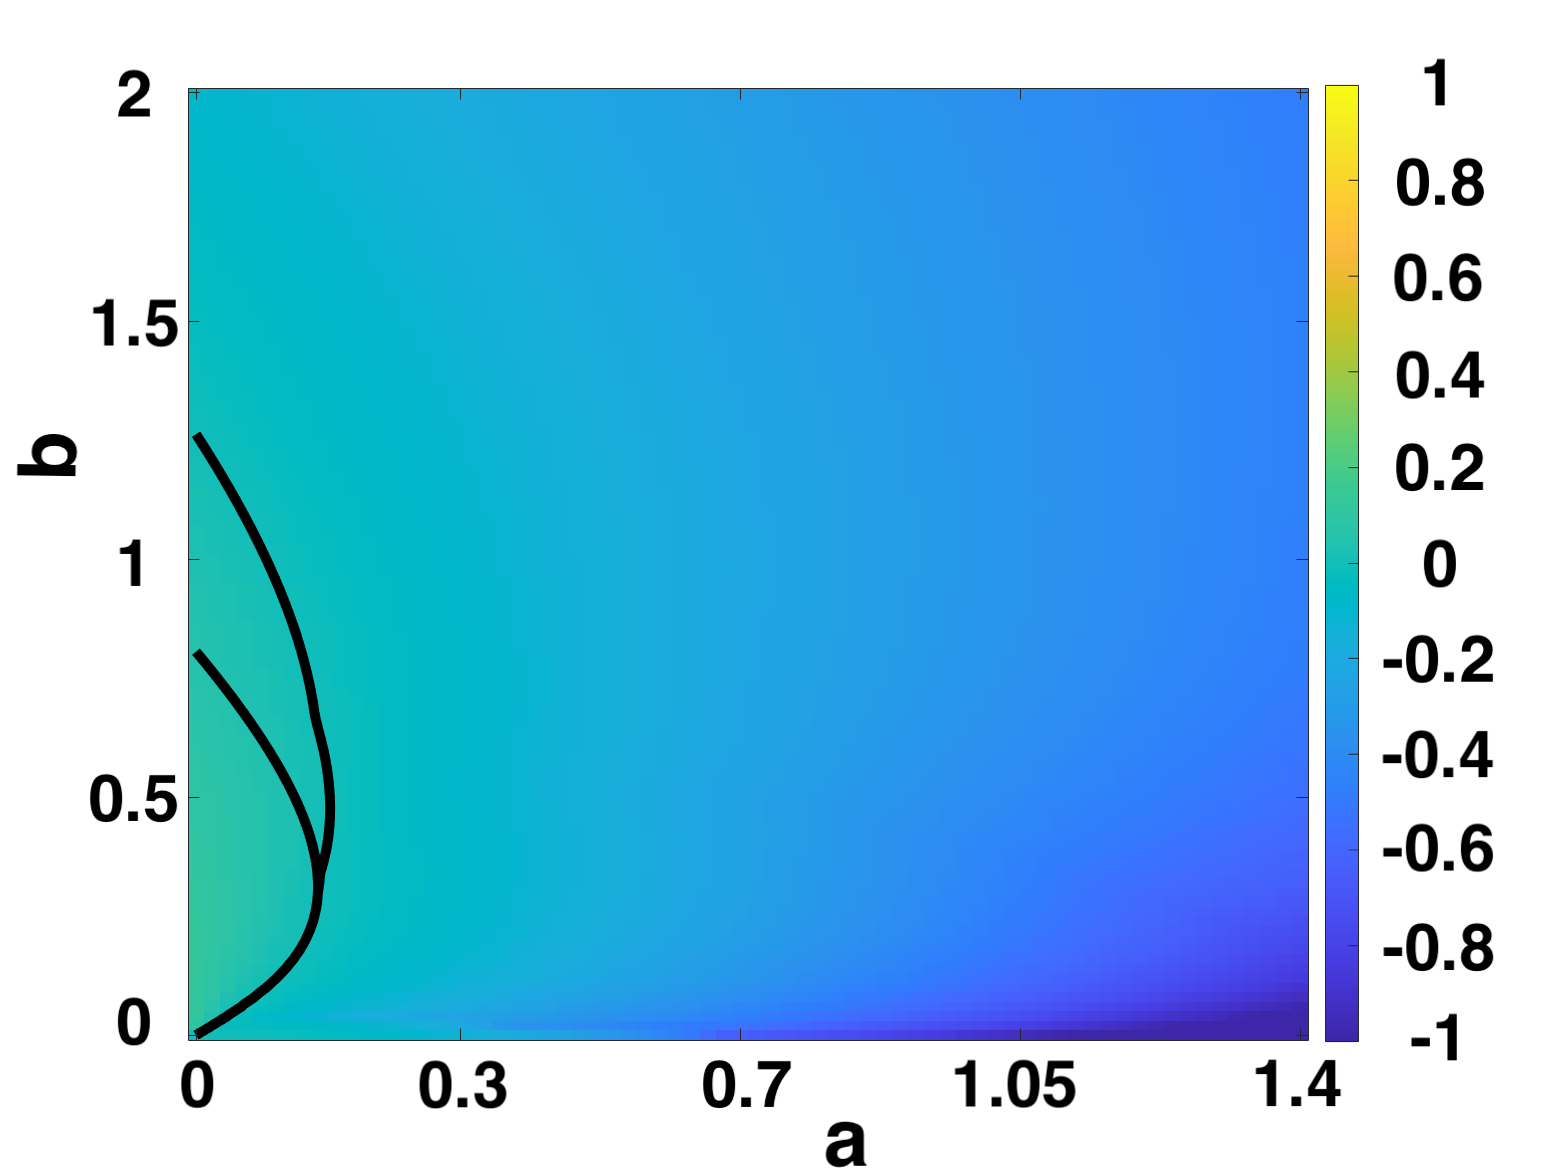
\includegraphics[width=7cm,height=5cm]{fixbif23.png}
        \caption{$\tau=1$}
        \label{}
    \end{subfigure}
    \hfill
    \begin{subfigure}[b]{0.45\textwidth}
        \centering
        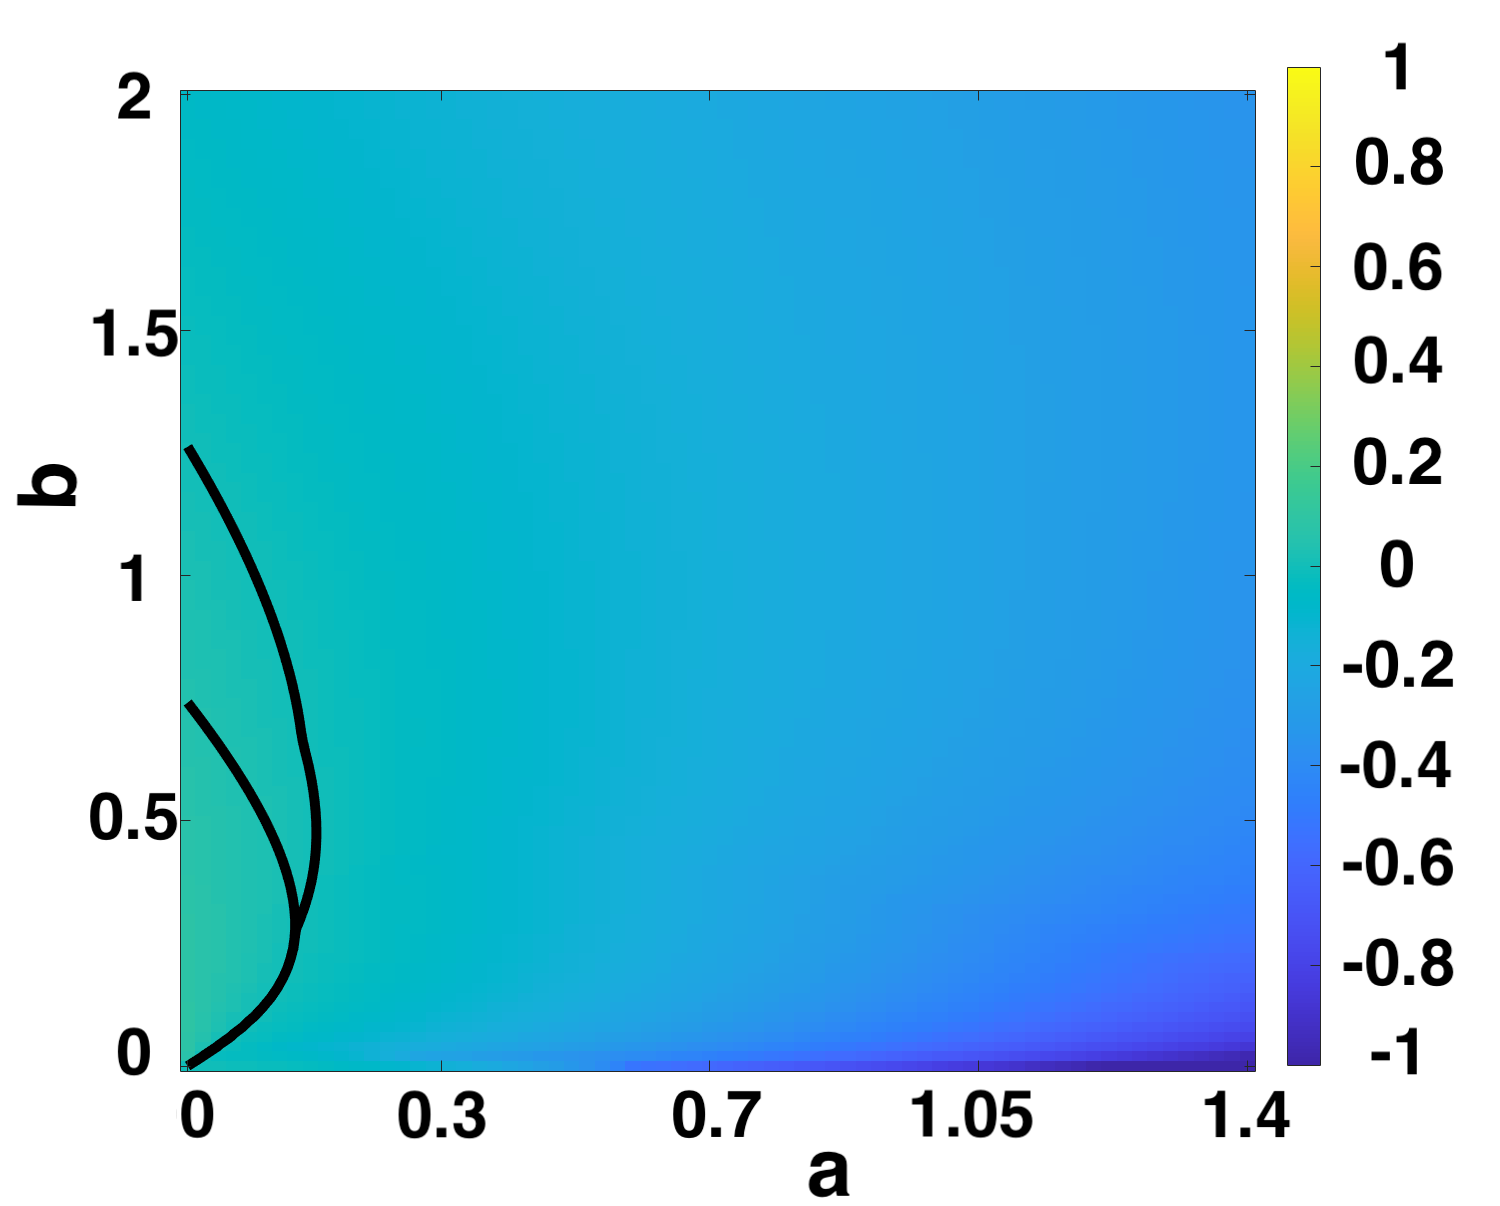
\includegraphics[width=7cm,height=5cm]{fixbif24.png}
        \caption{$\tau=1.5$.}
        \label{}
    \end{subfigure}
    \caption{$\max_k(\Re(\lambda_k))$ computed over $(a,b)$ parameter space, with $\epsilon^2=0.1$. As $\tau$ increases, $|\max_k(\Re(\lambda_k))|$ decreases.}
    \label{fig:fixbif2}
\end{figure}


\section{Investigation of Variation in Initial and Boundary Conditions}
In this section the robustness of the results obtained in \cite{gaffmonk} are examined under varying of initial conditions and boundary conditions. The results shown in this section are produced on a domain length $\Omega=[0,30]$. We first consider the sensitivity of pattern formation in the context of fixed time-delay to varying initial conditions. Three different sets of initial conditions are considerd. $\text{IC}_1$ corresponds to the intitial conditions used in \cite{gaffmonk}. The functional form of $\text{IC}_1$ can be found in Appendix \ref{appendix:extramath}. The following are the forms of the remaining initial conditions used

\begin{align}
\text{IC}_2&:\quad\quad\quad\begin{pmatrix}u_0\\v_0\end{pmatrix}=\begin{pmatrix}u_\star(1+r)\\v_\star(1+r)\end{pmatrix}\quad r\sim\mathcal{N}(0,0.01)\\
\text{IC}_3&:\quad\quad\quad\begin{pmatrix}u_0\\v_0\end{pmatrix}=\begin{pmatrix}u_\star(1+r)\\v_\star(1+r)\end{pmatrix}\quad r\sim\mathcal{N}(0,0.1)
\end{align}
The model parameters used match those used in \cite{gaffmonk}, with $(a,b)=(0.1,0.9)$, and a constant history function equal to the initial conditions was used. The results in \ref{fig:figtau0}, \ref{fig:figtau1}, \ref{fig:figtau2}, \ref{fig:figtau4}, and \ref{fig:figtau8} show the pattern formation observed for each of the initial conditions for varying fixed time-delay $\tau\in\{0,1,2,4,8 \}$.

\begin{figure}[H]
    \centering
    \begin{subfigure}[b]{0.32\textwidth}
        \centering
        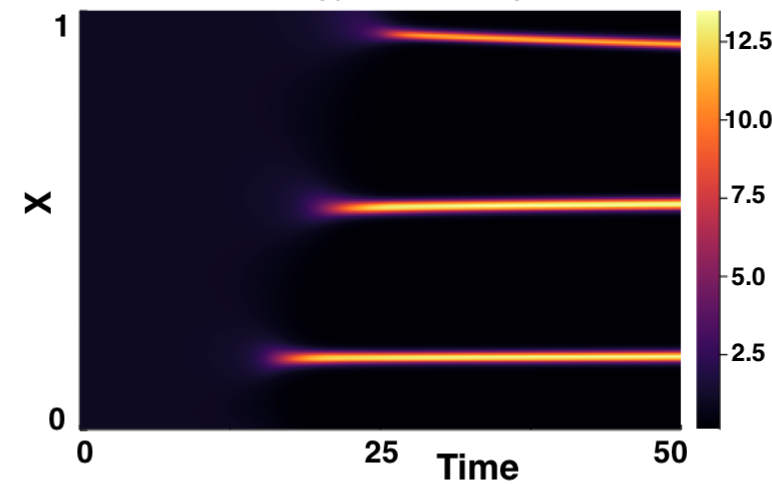
\includegraphics[width=5.5cm,height=4.5cm]{gaff0.png}
        \caption{$\text{IC}_1$}
        \label{}
    \end{subfigure}
    \hfill
    \begin{subfigure}[b]{0.32\textwidth}
        \centering
        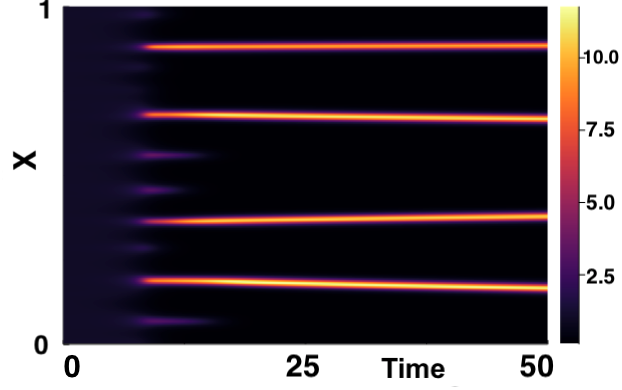
\includegraphics[width=5.5cm,height=4.5cm]{ic20.png}
        \caption{$\text{IC}_2$}
        \label{}
    \end{subfigure}
    \hfill
    \begin{subfigure}[b]{0.32\textwidth}
        \centering
        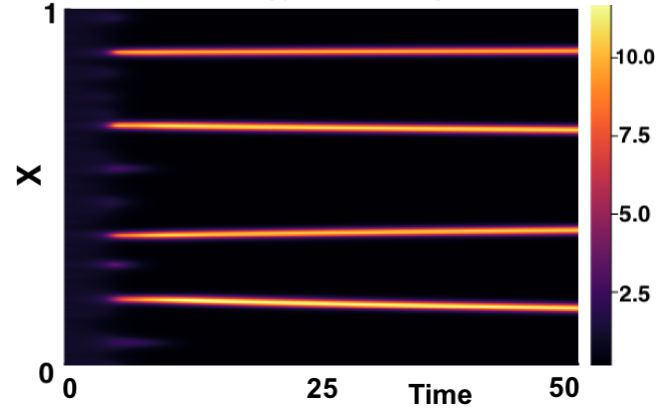
\includegraphics[width=5.5cm,height=4.5cm]{ic30.png}
        \caption{$\text{IC}_3$}
        \label{}
    \end{subfigure}
    \caption{Comparison of varying ICs for $\tau=0$}
    \label{fig:figtau0}
\end{figure}
\begin{figure}[H]
    \centering
    \begin{subfigure}[b]{0.32\textwidth}
        \centering
        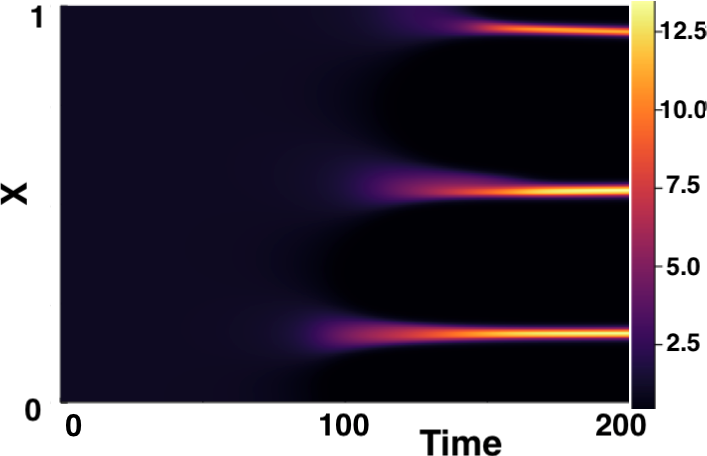
\includegraphics[width=5.5cm,height=4.5cm]{gaff1.png}
        \caption{$\text{IC}_1$}
        \label{}
    \end{subfigure}
    \hfill
    \begin{subfigure}[b]{0.32\textwidth}
        \centering
        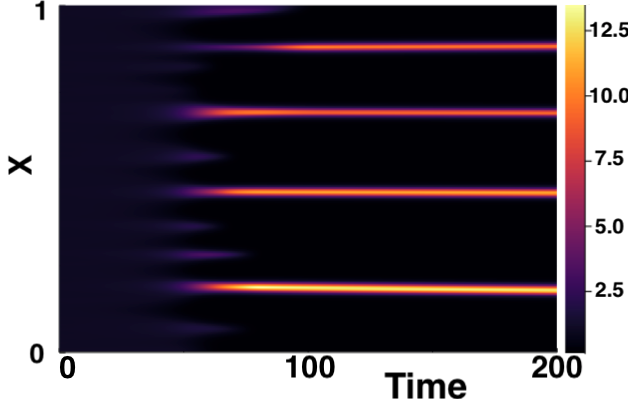
\includegraphics[width=5.5cm,height=4.5cm]{ic21.png}
        \caption{$\text{IC}_2$}
        \label{}
    \end{subfigure}
    \hfill
    \begin{subfigure}[b]{0.32\textwidth}
        \centering
        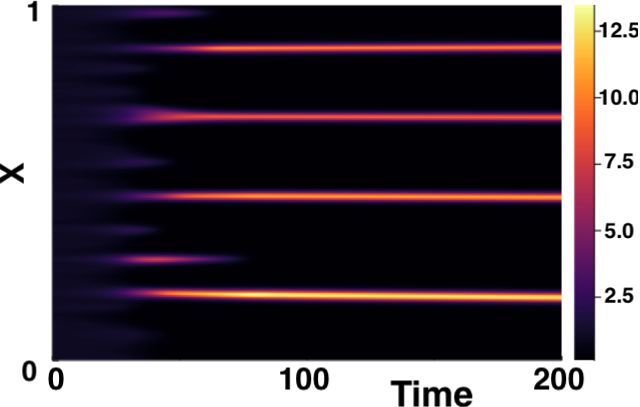
\includegraphics[width=5.5cm,height=4.5cm]{ic31.png}
        \caption{$\text{IC}_3$}
        \label{}
    \end{subfigure}
    \caption{Comparison of varying ICs for $\tau=1$}
    \label{fig:figtau1}
\end{figure}
\begin{figure}[H]
    \centering
    \begin{subfigure}[b]{0.32\textwidth}
        \centering
        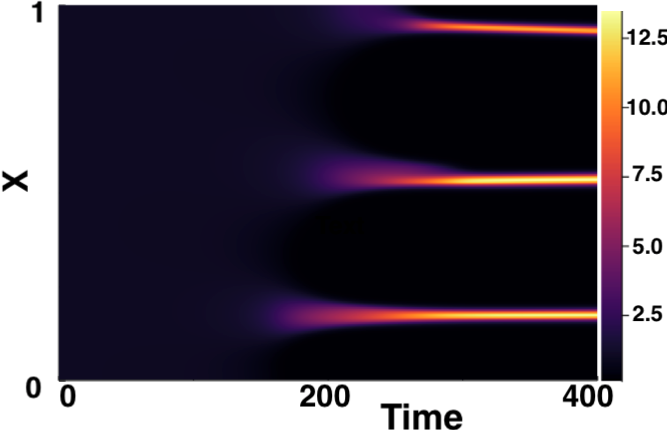
\includegraphics[width=5.5cm,height=4.5cm]{gaff2.png}
        \caption{$\text{IC}_1$}
        \label{}
    \end{subfigure}
    \hfill
    \begin{subfigure}[b]{0.32\textwidth}
        \centering
        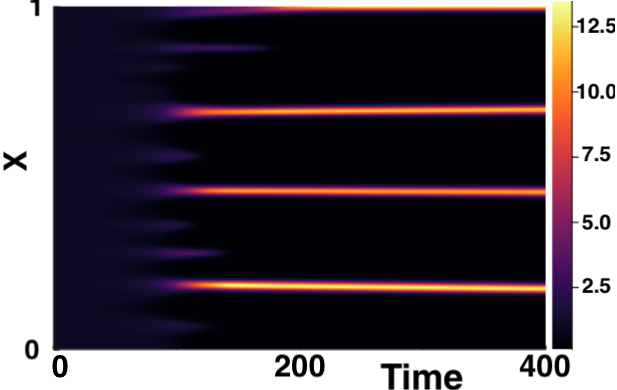
\includegraphics[width=5.5cm,height=4.5cm]{ic22.png}
        \caption{$\text{IC}_2$}
        \label{}
    \end{subfigure}
    \hfill
    \begin{subfigure}[b]{0.32\textwidth}
        \centering
        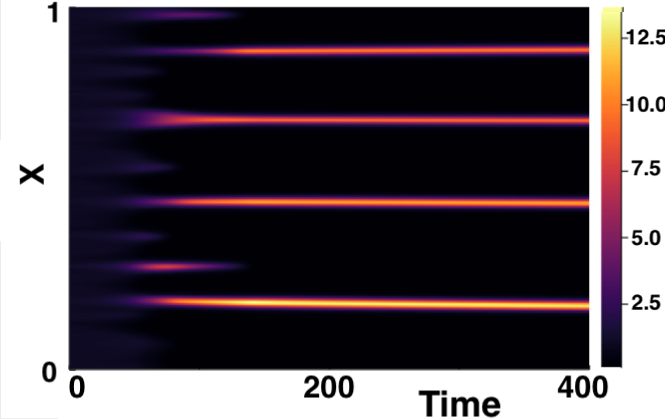
\includegraphics[width=5.5cm,height=4.5cm]{ic32.png}
        \caption{$\text{IC}_3$}
        \label{}
    \end{subfigure}
    \caption{Comparison of varying ICs for $\tau=2$}
    \label{fig:figtau2}
\end{figure}
\begin{figure}[H]
    \centering
    \begin{subfigure}[b]{0.32\textwidth}
        \centering
        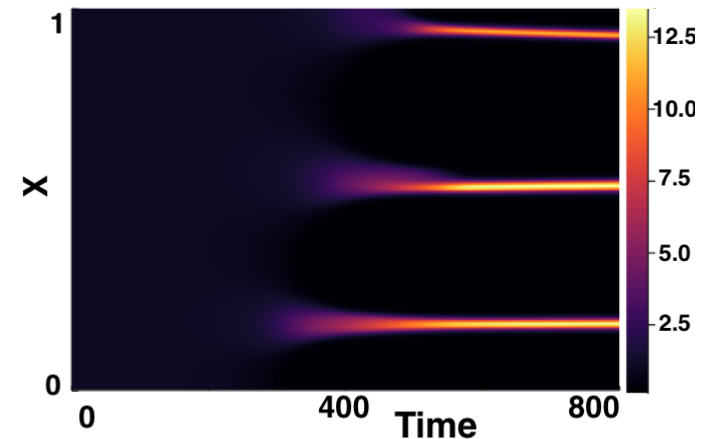
\includegraphics[width=5.5cm,height=4.5cm]{gaff4.png}
        \caption{$\text{IC}_1$}
        \label{}
    \end{subfigure}
    \hfill
    \begin{subfigure}[b]{0.32\textwidth}
        \centering
        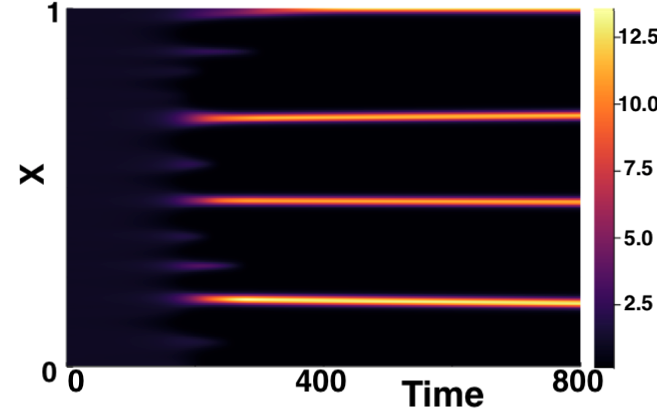
\includegraphics[width=5.5cm,height=4.5cm]{ic24.png}
        \caption{$\text{IC}_2$}
        \label{}
    \end{subfigure}
    \hfill
    \begin{subfigure}[b]{0.32\textwidth}
        \centering
        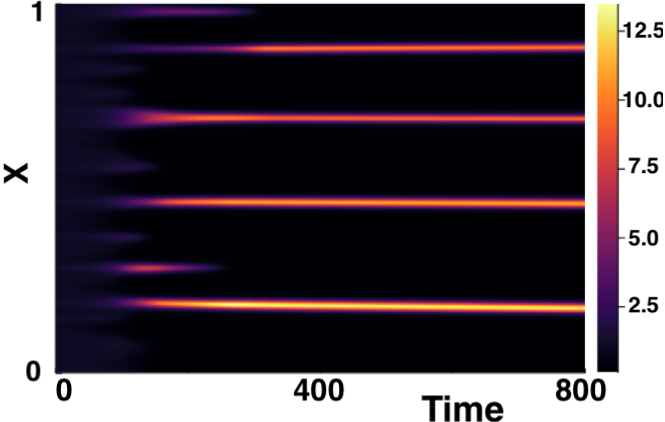
\includegraphics[width=5.5cm,height=4.5cm]{ic34.png}
        \caption{$\text{IC}_3$}
        \label{}
    \end{subfigure}
    \caption{Comparison of varying ICs for $\tau=4$}
    \label{fig:figtau4}
\end{figure}
\begin{figure}[H]
    \centering
    \begin{subfigure}[b]{0.32\textwidth}
        \centering
        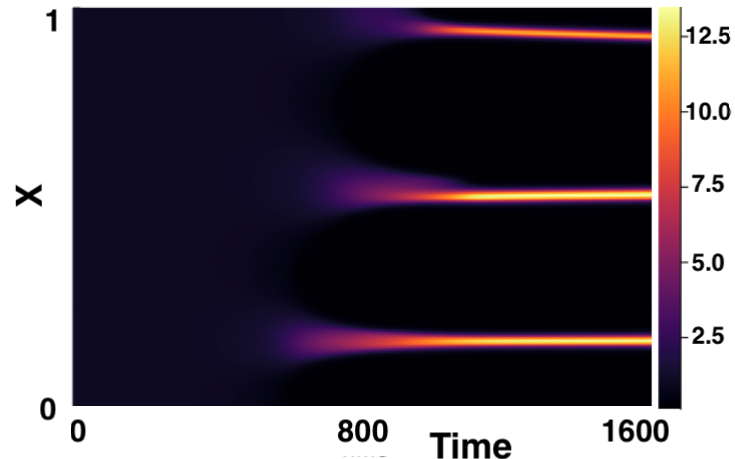
\includegraphics[width=5.5cm,height=4.5cm]{gaff8.png}
        \caption{$\text{IC}_1$}
        \label{}
    \end{subfigure}
    \hfill
    \begin{subfigure}[b]{0.32\textwidth}
        \centering
        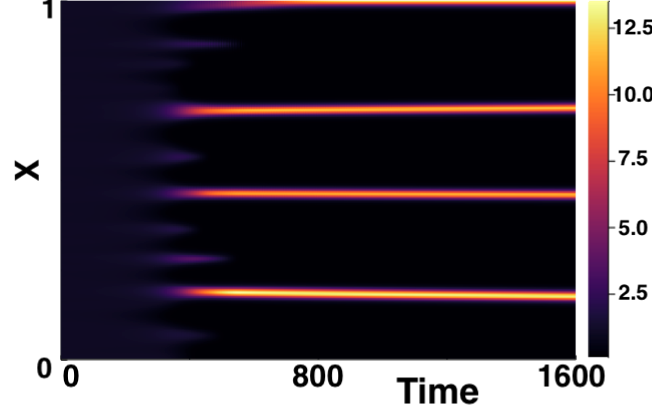
\includegraphics[width=5.5cm,height=4.5cm]{ic28.png}
        \caption{$\text{IC}_2$}
        \label{}
    \end{subfigure}
    \hfill
    \begin{subfigure}[b]{0.32\textwidth}
        \centering
        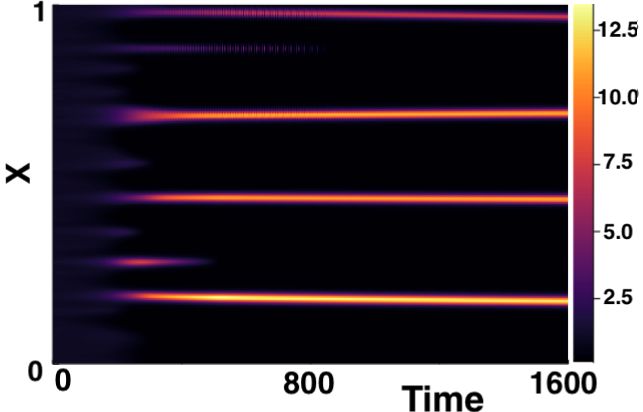
\includegraphics[width=5.5cm,height=4.5cm]{ic38.png}
        \caption{$\text{IC}_3$}
        \label{}
    \end{subfigure}
    \caption{Comparison of varying ICs for $\tau=8$}
    \label{fig:figtau8}
\end{figure}

It can be seen that the choice of initial conditions when considering the effect of time-delay on Turing pattern formation is exremely important. The choice of a random Gaussian perturbation rather than the functional form given in $\text{IC}_1$ also results in four `spikes' in the solution, rather than three. We also observe, for all initial condititions used, an approximate linear relationship between $\tau$ and the time-taken for pattern formation to occur. As $\tau$ is doubled the time-taken for the pattern to form is almost doubled. We also note from figures \ref{fig:figtau2}, \ref{fig:figtau4} and \ref{fig:figtau8}, that in the case of $\text{IC}_2$ and $\text{IC}_3$, as $\tau$ increases above $\tau=2$, the number of dominating modes in the pattern on the domain $[0,30]$ seems to shift from four to three, with the fourth spike appearing at the adge of the domain.
 We now consider the effect that variation in the history function may have on pattern formation.
\\
\\
INSERT FIGURES HERE
\\
\\
Finally, we consider the effect of varying boundary conditions. Motivated from the anlaysis in \cite{krausemixed}, homogeneous Dirichlet boundary conditions are implemented for the activator term, and homogeneous Neumann boundary conditions implemented for the inhibitor term. Thus, we have that, on a domain $\Omega=[0,L]$, $u=0$ and $\frac{\partial v}{\partial t}=0$ at $x=0, L$. These conditions are implemented numerically following the methodology outlined in section \ref{section:numimp}. The results in figures \ref{fig:bctau1}, \ref{fig:bctau2}, and \ref{fig:bctau3} were generated using $\text{IC}_2$, with a varying $\tau\in\{0,1,2\}$, and show the comparison between numerical simulations generated with homogeneous Neumann conditions for both $u$ and $v$, indicated as $\text{BC}_1$, and those generated with homogeneous Dirichlet conditions for $v$, indicated as $\text{BC}_2$.

\begin{figure}[H]
    \centering
    \begin{subfigure}[b]{0.45\textwidth}
        \centering
        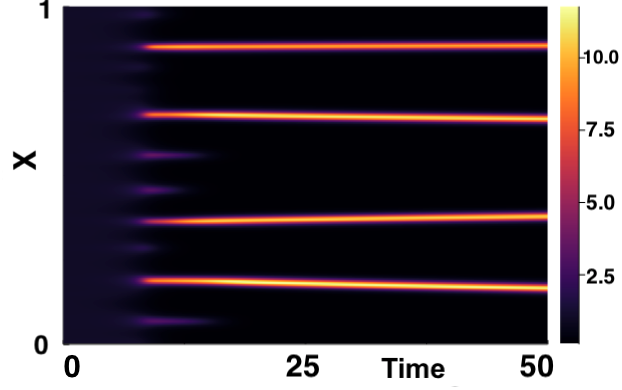
\includegraphics[width=7cm,height=5.5cm]{ic20.png}
        \caption{$\text{BC}_1$}
        \label{}
    \end{subfigure}
    \hfill
    \begin{subfigure}[b]{0.45\textwidth}
        \centering
        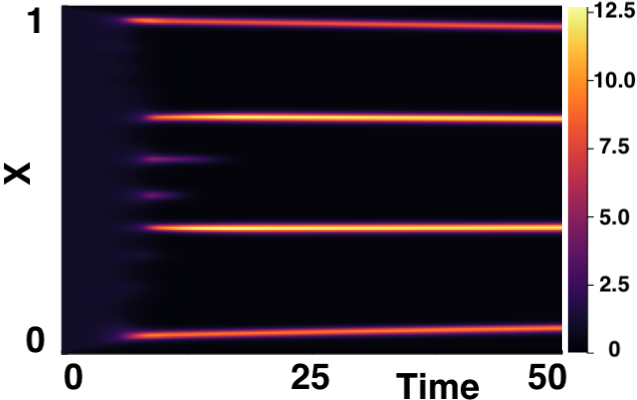
\includegraphics[width=7cm,height=5.5cm]{bc0.png}
        \caption{$\text{BC}_2$}
        \label{}
    \end{subfigure}
    \caption{Comparison of varying BCs for $\tau=0$. Generated with $\text{IC}_2$}
    \label{fig:bctau1}
\end{figure}

\begin{figure}[H]
    \centering
    \begin{subfigure}[b]{0.45\textwidth}
        \centering
        \includegraphics[width=7cm,height=5.5cm]{ic21.png}
        \caption{$\text{BC}_1$}
        \label{}
    \end{subfigure}
    \hfill
    \begin{subfigure}[b]{0.45\textwidth}
        \centering
        \includegraphics[width=7cm,height=5.5cm]{bc1.png}
        \caption{$\text{BC}_2$}
        \label{}
    \end{subfigure}
    \caption{Comparison of varying BCs for $\tau=1$. Generated with $\text{IC}_2$}
    \label{fig:bctau2}
\end{figure}

\begin{figure}[H]
    \centering
    \begin{subfigure}[b]{0.45\textwidth}
        \centering
        \includegraphics[width=7cm,height=5.5cm]{ic22.png}
        \caption{$\text{BC}_1$}
        \label{}
    \end{subfigure}
    \hfill
    \begin{subfigure}[b]{0.45\textwidth}
        \centering
        \includegraphics[width=7cm,height=5.5cm]{bc2.png}
        \caption{$\text{BC}_2$}
        \label{}
    \end{subfigure}
    \caption{Comparison of varying BCs for $\tau=2$. Generated with $\text{IC}_2$}
    \label{fig:bctau3}
\end{figure}

\section{Relationship Between Time-To-Pattern and Time-Delay}\label{section:delaypatt}

We aim to show that, for small $\tau$ and domain $\Omega$, the linear theory provides a good approximation to the time-taken until pattern formation occurs, and in fact, the relationship between $\tau$ and time-to-pattern under these conditions is linear.
In order to minimise the effect of nonlinearity in the dynamics, we restrict the domain size to $\Omega=[0,2]$. Shrinking the domain results in fewer unstable modes at lower frequencies and thus less competition for the dominant mode at higher frequencies, resulting in a better approximation of the linear theory. This finite size effect can be seen in figure \ref{fig:compardisp}, where $\Re(\lambda_k)$ is plotted against $k$ for two different domain sizes, for a given $(a,b,\tau)$. Due to numerical restrictions in finding roots of the characteristic equation \eqref{characfix}, only $\tau\leq1.6$ is considered. Similar to the initial conditions used for previous numerical simulations (figure \ref{fig:fixedsim2}), we take a small perturbation in the activator term, $\hat{u}(t)$, such that $\hat{u}(0)=ru_\star$, where $r$ is a small Gaussian random variable, $r\sim\mathcal{N}(0,\sigma^2)$,
for some standard deviation $\sigma$. The linear theory suggests that at some time $t=T$, the perturbation will be of the form $\hat{u}(T)\sim A_k(T)\cos\left(\frac{k\pi x}{L}\right)$, where $k$ is the dominant mode, $\lambda_k$ is the corresponding eigenvalue, or growth rate, and $A_k(T)$ denotes the corresponding fourier coefficient at time $t=T$. For a given parameter set $(a,b,\epsilon^2,\tau,L)$, we can solve the characteristic equation \eqref{characfix}, and plot $\Re(\lambda_k)$
against $k$, to determine the dominating mode $k$ and the corresponding $\lambda_k$. We then use this information in the following manner: we use a fast fourier transform to decompose the intitial conditions into a fourier series, and compute the coefficient $A_k(0)$ for the dominating $k$. When the perturbation $\hat{u}$ has grown sufficiently, in absolute value, beyond a threshold where pattern formation is considered, we call this time $t=T$, and again determine the fourier coefficient $A_k(T)$ of the fastest growing mode $k$. Using the relation $A_k(T)\sim A_k(0)e^{\lambda_k T}$, we rearrange for $T$ and thus compute a linear approximation for time-to-pattern as
\begin{equation}
    T=\frac{1}{\lambda_k}\ln\left(\frac{A_k(T)}{A_k(0)}\right).
\end{equation}
The standard deviation for the random variable $r$ is given as $\sigma=10^-5$, and the threshold value at $0.1$. A very small perturbation was used as a means to improve the accuracy of the linear theory.
\begin{figure}[H]
    \centering
    \begin{subfigure}[b]{0.45\textwidth}
        \centering
        \includegraphics[width=7cm,height=5.5cm]{compdisp1.png}
        \caption{Dispersion curve plotted with domain size $L=0.1$.}
        \label{fig:compdisp1}
    \end{subfigure}
    \hfill
    \begin{subfigure}[b]{0.45\textwidth}
        \centering
        \includegraphics[width=7cm,height=5.5cm]{compdisp2.png}
        \caption{Dispersion curve plotted with domain size $L=1.5$.}
        \label{fig:compdisp2}
    \end{subfigure}
    \caption{Dispersion curves plotted for $(a,b,\tau)=(0.4,1.8,0.2)$. A larger $L$ results in more unstable modes $\lambda_k$ such that $\Re(\lambda)>0$. }
    \label{fig:compardisp}
\end{figure}
On the domain $\Omega=[0, 0.1]$, figure \ref{fig:compdisp1} suggests that at $\tau=0.2$, from the linear theory, the dominant mode is $k=1$. Figure \ref{fig:icfc} shows the initial condition used, with random perturbation described as above, and the plotted Fourier coefficients $A_k(0)$, in absolute value, for $k\neq0$.
\begin{figure}[H]
    \centering
    \begin{subfigure}[b]{0.45\textwidth}
        \centering
        \includegraphics[width=8.5cm,height=6cm]{uic.png}
        \caption{Initial conditions of activator $u$ across spatial domain.}
        \label{}
    \end{subfigure}
    \hfill
    \begin{subfigure}[b]{0.45\textwidth}
        \centering
        \includegraphics[width=8.5cm,height=6cm]{uicfc.png}
        \caption{Absolute Fourier coefficients, $|A_k(0)|$, of initial conditions, $k\neq0$.}
        \label{fig:}
    \end{subfigure}
    \caption{Initial conditions as a small Gaussian perurbation of $O(10^{-5})$. Fourier coefficients $A_k(0)$ computed using Fast Fourier Transform.}
    \label{fig:icfc}
\end{figure}
Since $k=1$ is the dominant mode, we extract the first Fourier coefficient of the initial conditions, $A_1(0)$, as $A_1(0)=7.95(3.s.f)\times10^{-8}$. To find $A_1(T)$, a numerical simulation is run until the perturbation of $O(10^-5)$ as grown, in absolute values, to a threshold value of $0.1$. Simulating first for a time delay $\tau=0.2$, figure \ref{fig:Tfc} shows the numerical solution $u(T)$ at the point where the perturbation has grown to this threshold value, as well as a scatter plot of the Fourier coefficients $A_k(T)$, $k\neq0$.
\begin{figure}[H]
    \centering
    \begin{subfigure}[b]{0.45\textwidth}
        \centering
        \includegraphics[width=8.5cm,height=6cm]{Tu.png}
        \caption{Numerical solution $u(T)$ at $t=T$}
        \label{uT}
    \end{subfigure}
    \hfill
    \begin{subfigure}[b]{0.45\textwidth}
        \centering
        \includegraphics[width=8.5cm,height=6cm]{Tfc.png}
        \caption{Absolute Fourier coefficients, $|A_k(T)|$, of $u(T)$.}
        \label{fig:uTfc}
    \end{subfigure}
    \caption{}
    \label{fig:Tfc}
\end{figure}
As seen in figure \ref{fig:uTfc}, the Fourier coefficient of the first, and dominant, mode is given as $0.0262(3.s.f)$. Using the dispersion plot in figure \ref{fig:compdisp1}, the corresponding dominant eigenvalue $\lambda_1$ is found as $\lambda_1=0.236(3.s.f)$. The approximated time-to-pattern, as predictied by linear theory, for $(a,b,\tau)=(0.4,1.8,0.2)$ and the given initial conditions is thus computed as
\begin{equation}
    T=\frac{1}{\lambda_1}\ln\left(\frac{A_1(T)}{A_1(0)}\right)=\frac{1}{0.2356}\ln\left(\frac{0.0262}{7.95\times10^{-8}}\right)=53.8(3.s.f).
\end{equation}
It was found through numerical solution that the `true' time-to-pattern is $\approx57.5(3sf)$. The numerical solution for a timespan $t\in[0,80]$ can be seen in figure \ref{fig:dispnumsim}. The process above can be repeated for varying $(a,b,\tau)$, and figures \ref{fig:ttp1}, \ref{fig:ttp2}, \ref{fig:ttp3} show the predicted time-to-pattern plotted against $\tau$ and compared with the `true' time-to-pattern for three different parameter sets. The time-delay is varied here over $\tau\in[0,1.6]$.

\begin{figure}[H]
    \centering
    \begin{subfigure}[b]{0.45\textwidth}
        \centering
        \includegraphics[width=8.5cm,height=6cm]{dispnumsim.png}
        \caption{Numerical solution for $(a,b,\tau)=(0.4,1.8,0.2)$}
        \label{fig:dispnumsim}
    \end{subfigure}
    \hfill
    \begin{subfigure}[b]{0.45\textwidth}
        \centering
        \includegraphics[width=8.5cm,height=6cm]{ttp1.png}
        \caption{Predicted vs `true' time-to-pattern for $(a,b)=(0.4,1.8)$.}
        \label{fig:ttp1}
    \end{subfigure}
    \caption{}
    \label{}
\end{figure}

\begin{figure}[H]
    \centering
    \begin{subfigure}[b]{0.45\textwidth}
        \centering
        \includegraphics[width=8.5cm,height=6cm]{ttp2.png}
        \caption{Predicted vs `true' time-to-pattern for $(a,b)=(0.1,0.9)$.}
        \label{fig:ttp2}
    \end{subfigure}
    \hfill
    \begin{subfigure}[b]{0.45\textwidth}
        \centering
        \includegraphics[width=8.5cm,height=6cm]{ttp3.png}
        \caption{Predicted vs `true' time-to-pattern for $(a,b)=(0.2,1.3)$.}
        \label{fig:ttp3}
    \end{subfigure}
    \caption{}
    \label{}
\end{figure}

\newpage
\chapter{Distributed Delay Model}

In the previous chapter we introduced a fixed constant delay into the dynamics of the activator. The stochastic nature of gene expression delays lead us however to consider a mean-field approach to modelling the time delay \cite{bratsun,krausenew}. As done in \cite{william}, by assuming each individual mechanism within the gene expression process acts independently and identically, we use the central limit theorem to model the delay as Gaussian distribution with some mean $\tau$ and standard deviation $\sigma$. We begin by using a symmetric truncated Guassian distribuion, with integration limits $a=\tau-n\sigma$ and $b=\tau+n\sigma$ for some $n\in\mathbb{N}$, such that $a=\tau-n\sigma>0$ to maintain positive time delays. We can thus write the LI model with distributed time delay as

\begin{equation}
  \begin{split}
    \frac{\partial u}{\partial t}&=\frac{\epsilon^2}{\gamma}\frac{\partial^2u}{\partial x^2}+a-u-2u^2v+3\int_{a}^{b}k(s,\tau,\sigma)\hat{u}^2\hat{v} \quad\text{ds},\\
    \frac{\partial v}{\partial t}&=\frac{1}{\gamma}\frac{\partial^2v}{\partial x^2}+b-u^2v,
\end{split}
\end{equation}
where $\hat{u}=u(x,t-s)$ and $\hat{v}=v(x,t-s)$ where $s$ is the integration variable ranging over the delays. $k(s,\tau,\sigma)$ is the truncated Gaussian pdf and for some mean $\tau$ and standard devation $\sigma$ is given by \cite{wikitrunc}

\begin{equation}
  k(s)=\frac{\Phi_c}{\sqrt{2\pi}\sigma}\exp\left(\frac{-1}{2}\left(\frac{s-\tau}{\sigma}\right)^2\right).
\end{equation}
We use $\Phi_c$ to denote the truncation scaling constant. This constant ensures $k(s,\tau,\sigma)$ integrates to $1$ over the given integration domain $[a, b]$, and is computed as
\begin{equation}
\Phi_c=\frac{1}{\phi\left(\frac{b-\tau}{\sigma}\right)-\phi\left(\frac{a-\tau}{\sigma}\right)},
\end{equation}
with the function $\phi$ described by
\begin{equation}
\phi(x)=\frac{1}{2}\left(1+\text{erf}\left(\frac{x}{\sqrt{2}}\right)\right).
\end{equation}
In order to simulate the distributed delay model, we will use the composite Simpson's quadrature rule to numerically resolve the integral term \cite{compsimp}. Convergence analysis of the quadrature rule will be considered in section \ref{section:quad}.

\subsection{Quadrature}\label{section:quad}
The integration domain $[a, b]$, with $a=\tau-n\sigma$ and $b=\tau+n\sigma$, can be discretised into $N$ sub-intervals of equal length with $N+1$ discretisation points, $s_0,\cdots,s_{N}$, such that $s_0=\tau-n\sigma$ and $s_N=\tau+n\sigma$. Using the composite Simpsons's rule \cite{compsimp}, the integral term can be numerically approximated as

\begin{equation}\label{simp}\int_{a}^{b}k(s)\hat{u}^2\hat{v}\  \text{ds}\approx\frac{h}{3}\left[k(s_0)\hat{u}^2_0\hat{v}_0+2\sum_{i=1}^{\frac{N}{2}-1}k(s_{2i})\hat{u}^2_{2i}\hat{v}_{2i}+4\sum_{i=2}^{\frac{N}{2}}k(s_{2i-1})\hat{u}^2_{2i-1}\hat{v}_{2i-1}+k(s_N)\hat{u}^2_N\hat{v}_N\right],
\end{equation}
where $h$ is computed as $h=\frac{b-a}{N}$. We use the notation $\hat{u}_j$ and $\hat{v}_j$ to denote $u(t-s_j)$ and $v(t-s_j$) respectively, namely the functions $u$ and $v$ evaluated at time-delay with some index $j$, $s_j$. Throughout the report we use $n=3$, so that the integration limits are $a=\tau-3\sigma$ and $b=\tau+3\sigma$. This was chosen so that a relatively large $\sigma$ value could be chosen for each $\tau$ while maintaining $a>0$.
Figures \ref{fig:pdf1} and \ref{fig:pdf2} show the pdf of a truncated Gaussian distribution centred at a mean $\tau=1,2$ with varying $\sigma$ values as fractions of $\sigma_{max}$. We have $s$ as the integration variable, with $s\in[a,b]$.

\begin{figure}[H]
    \centering
    \begin{subfigure}[b]{0.45\textwidth}
        \centering
        \includegraphics[width=7cm,height=5cm]{t1sig1.png}
        \caption{Truncated Gaussian distribution following $\mathcal{N}(1,(\sigma_{max}\times0.99)^2)$}
        \label{}
    \end{subfigure}
    \hfill
    \begin{subfigure}[b]{0.45\textwidth}
        \centering
        \includegraphics[width=7cm,height=5cm]{t1sig2.png}
        \caption{Truncated Gaussian distribution following $\mathcal{N}(1,(\sigma_{max}\times0.1)^2)$}
        \label{}
    \end{subfigure}
\caption{PDF of truncated Gaussian distribution with mean $\tau=1$ and integration domain $[1-3\sigma,1+3\sigma]$.}
\label{fig:pdf1}
\end{figure}
\begin{figure}[H]
    \centering
    \begin{subfigure}[b]{0.45\textwidth}
        \centering
        \includegraphics[width=7cm,height=5cm]{t2sig1.png}
        \caption{Truncated Gaussian distribution following $\mathcal{N}(2,(\sigma_{max}\times0.99)^2)$}
        \label{}
    \end{subfigure}
    \hfill
    \begin{subfigure}[b]{0.45\textwidth}
        \centering
        \includegraphics[width=7cm,height=5cm]{t2sig2.png}
        \caption{Truncated Gaussian distribution following $\mathcal{N}(2,(\sigma_{max}\times0.1)^2)$}
        \label{}
    \end{subfigure}
    \caption{PDF of truncated Gaussian distribution with mean $\tau=2$ and integration domain $[2-3\sigma,2+3\sigma]$.}
    \label{fig:pdf2}
\end{figure}
We see that $\sigma$ is responsible for scaling on the $x$-axis, while the truncation constant $\Phi_c$ scales the $y$-axis, ensuring the pdf integrates to $1$ across the integration domain. For the implementation of the quadrature rule, the number of sub-intervals $N$ was chosen to be $N=50$. The consideration for such a choice involves both quadrature accuracy and computational efficiency. The motivation for setting $N=50$ was dependant on evaluating `test' integrals and simulation `test' DDEs, for which the results are presented in the remainder of this section.

\section{Linear Analysis}\label{section:distlin}
The system of equations is given by
\begin{equation}\label{dist}
  \begin{split}
  \frac{\partial u}{\partial t}&=D_u\frac{\partial^2u}{\partial x^2}+a-u-2u^2v+3\int_a^bk(s)\hat{u}^2\hat{v} \text{ds}\\
  \frac{\partial v}{\partial t}&=D_v\frac{\partial^2v}{\partial x^2}+b-u^2v,
\end{split}
\end{equation}
where $u=u(x,t)$, $v=v(x,t)$, $\hat{u}=u(x,t-s)$ and $\hat{v}=v(x,t-s)$. $k(s)$ is the truncated Gaussian distribution, integrating to $1$ between constant limits $a$ and $b$, and is given by
\begin{equation}
k(s)=\frac{\Phi_c}{\sqrt{2\pi}\sigma}\exp\left(\frac{-1}{2}\left(\frac{s-\tau}{\sigma}\right)^2\right),
\end{equation}
for some mean $\tau$ and standard deviation $\sigma$. $\Phi_c$ denotes the truncation scaling factor. Denoting the steady-state $(u_\star,v_\star)$, and taking a small perturbation about the steady-state $u=u_\star+\epsilon\xi$, $v=v_\star+\epsilon\eta$, where $|\epsilon|\ll1$, we can write the equation for $u$ in \eqref{dist} as

\begin{equation}\label{perturb}
  \epsilon\frac{\partial \xi}{\partial t}=\epsilon D_u\frac{\partial^2\xi}{\partial x^2}+f(u_\star+\epsilon\xi, v_\star+\epsilon\eta)+g(u_\star+\epsilon\hat{\xi},v_\star+\epsilon\hat{\eta}) ,
\end{equation}
where $f(u,v)=a-u+2u^2v$ and $g(\hat{u},\hat{v})=3\int_a^bk(s)\hat{u}^2\hat{v} \text{ds}$. The $\hat{\xi}$ notation is used to denote the perturbation evaluated at a delay $\hat{\xi}=\xi(x,t-s)$. Taylor expanding equation \eqref{perturb} for the $f$ term about the steady-state and evaluating the $g$ term, up to $O(\epsilon)$, yields

\begin{dmath}\label{taylor}
  \epsilon\frac{\partial \xi}{\partial t}=\epsilon D_u\frac{\partial^2\xi}{\partial x^2}+f(u_\star,v_\star)+3u_\star^2v_\star\int_a^bk(s)\text{ds}+\epsilon\left[\xi f_u(u_\star,v_\star)+\eta f_v(u_\star,v_\star)+6u_\star v_\star\int_a^bk(s)\hat{\xi}\text{ds}+3u_\star^2\int_a^bk(s)\hat{\eta}\text{ds}
  \right].
\end{dmath}
We use the notation $f_u$ to denote the derivative of function $f$ with respect $u$. Using the facts that the truncated Guassian $k(s)$ integrates to $1$ over $[a,b]$, and evaluation the expressions $f_u(u_\star,v_\star)$ and $f_v(u_\star,v_\star)$, equation \eqref{taylor} can be simplified to

\begin{equation}\label{linu}
  \epsilon \frac{\partial \xi}{\partial t}=\epsilon D_u\frac{\partial^2\xi}{\partial x^2}+\epsilon\left[\xi(-1-4u_\star v_\star)-2\eta u_\star^2 +6u_\star v_\star\int_a^bk(s)\hat{\xi}\text{ds}+3u_\star^2\int_a^bk(s)\hat{\eta}\text{ds}\right].
\end{equation}
The linearised dynmacs for $v$ are more simply given by
\begin{equation}\label{linv}
\epsilon \frac{\partial\eta}{\partial t}=\epsilon D_v\frac{\partial^2\eta}{\partial x^2}-\epsilon\left[2\xi u_\star v_\star+\eta u_\star^2\right].
\end{equation}
Substituting in an ansatz of the form $\xi=\xi_0e^{\lambda t}\cos(k\pi x)$ \cite{yigaffneyli} into \eqref{linu} and $\eta=\eta_0e^{\lambda t}\cos(k\pi x)$ into \eqref{linv}, and then dividing through by $e^{\lambda t}$ and $\cos(k\pi x)$, results in

\begin{equation}\label{sysof}
  \begin{split}
\lambda\xi_0&=-D_uk^2\pi^2\xi_0+\xi_0(-1-4u_\star v_\star)-2\eta_0u_\star^2+6\xi_0u_\star v_\star E+3\xi_0u_\star^2E \\
\lambda\eta_0&=-D_vk^2\pi^2\eta_0-2\xi_0u_\star v_\star-\eta_0u_\star^2,
\end{split}
\end{equation}
where $E=\int_a^bk(s)e^{-\lambda s}\text{ds}$. We can write equation \eqref{sysof} as a homogeneous linear system for $(\xi_0,\eta_0)^T$, given by

\begin{equation}
\underbrace{\begin{pmatrix}-1-4u_\star v_\star-D_uk^2\pi^2+6u_\star v_\star E-\lambda&-2u_\star^2+3u_\star^2E\\-2u_\star v_\star&-u_\star^2-D_vk^2\pi^2-\lambda \end{pmatrix}}_{\textbf{M}}\begin{pmatrix}\xi_0\\\eta_0\end{pmatrix}=\begin{pmatrix}0\\0\end{pmatrix}.
\end{equation}
Looking for non-trivial solutions, we look for roots of the characteristic equation, namely $D_k=\text{det}(\textbf{M})=0$. The characteristic equation, $D_k$, is given as
\begin{equation}\label{characdist}
  D_k=\lambda^2+\alpha_k\lambda+\beta_k+(\gamma_k\lambda+\delta_k)E=0,
\end{equation}
where
\begin{align}
\alpha_k&=(D_u+D_v)k^2\pi^2+u_\star^2+4u_\star v_\star+1\\
\beta_k&=(D_v\pi^2k^2+u_\star^2)(D_u\pi^2k^2+4u_\star v_\star+1)-4u_\star^3v_\star\\
\gamma_k&=-6u_\star v_\star\\
\delta_k&=-6D_vu_\star v_\star k^2\pi^2.
\end{align}

Finally, we note that the expression $E$ can be evaluated as
\begin{equation}
E=\int_a^bk(s)e^{-\lambda s}ds=\frac{\Phi_c}{2}\left[\exp\left(\frac{\lambda(\lambda\sigma^2-2\tau)}{2}\right) \text{erf} \left(\frac{\lambda\sigma^2+s-\tau}{\sqrt{2}\sigma}\right)\right]\Bigg|_a^b.
\end{equation}
The charactersitic equation \eqref{characdist} cannot trivially be split into it's real and imaginary components due to the error function term in $E$ as was done in the fixed delay case. We therefore cannot explicitly compute the stability lines in $(a,b)$ parameter space. We can however range over $(a,b)$ and compute $\max_k(\Re(\lambda_k))$ for different $\tau$, and produce plots similar to those in figures \ref{fig:dispfixed} and \ref{fig:lambdavary}. We use these plots to pseudo-analytically prove that, using a symmetric Gaussian distribution centred at mean $\tau$ will not change the time-to pattern seen for a fixed delay of $\tau$, independent of the standard deviation of the distribution $\sigma$. We first plot $\max_k(\Re(\lambda_k))$ against $\tau$, as seen analogously in figure \ref{fig:dispfixed} for the fixed delay case, for multiple parameters $(a,b,\tau,\sigma)$, and compares these to the fixed delay case. Since physically we cannot have negative delays, we require the lower integration limit to be positive. Namely, for a given mean $\tau$, we require $\tau-3\sigma>0$. We therefore define a maximum $\sigma$ value by $\sigma_{max}=\tau / 3$. By ensuring $\sigma<\sigma_{max}$, we ensure only positive delays are considered. Figures \ref{fig:p1}, \ref{fig:p2}, and \ref{fig:p3} show $\max_k(\Re(\lambda_k))$ plotted against $\tau\in[0,1]$ for three different parameter sets $(a,b)=\{(0.3,1.2), (0.1,0.9), (0.4,0.4)\}$. For each parameter set, plots are produced with different $\sigma$ values as a fraction of $\sigma_{max}$, as well as for the fixed delay case. We note that in the distributed delay case, as we vary $\tau$, $\sigma_{max}$ and thus the integration limits both change as functions of $\tau$. The domain length was again given by $L=30$, and $k$ varied from $[0,20]$ at regular discrete intervals of $1$.

% PARAMTER SET 1
\begin{figure}[H]
    \centering
    \begin{subfigure}[b]{0.45\textwidth}
        \centering
        \includegraphics[width=7cm,height=5cm]{p1fixed.png}
        \caption{Fixed delay case.}
        \label{}
    \end{subfigure}
    \hfill
    \begin{subfigure}[b]{0.45\textwidth}
        \centering
        \includegraphics[width=7cm,height=5cm]{p1sigmax.png}
        \caption{Distributed delay with $\sigma=\sigma_{max}\times0.99$.}
        \label{}
    \end{subfigure}
    \hfill
    \begin{subfigure}[b]{0.45\textwidth}
        \centering
        \includegraphics[width=7cm,height=5cm]{p1sigmax5.png}
        \caption{Distributed delay with $\sigma=\sigma_{max}\times0.2$.}
        \label{}
    \end{subfigure}
    \hfill
    \begin{subfigure}[b]{0.45\textwidth}
        \centering
        \includegraphics[width=7cm,height=5cm]{p1sigmax10.png}
        \caption{Distributed delay with $\sigma=\sigma_{max}\times0.1$.}
        \label{}
    \end{subfigure}
    \caption{$\max_k(\Re(\lambda_k))$ plotted against $\tau\in[0,1]$ for parameter set $(a,b,\epsilon^2)=(0.3,1.2,0.001)$. $\Omega=[0,30]$ and $k$ varied over $[0,20]$ at regular discrete intervals of $1$.}
    \label{fig:p1}
\end{figure}
% PARAMTER SET 2
\begin{figure}[H]
    \centering
    \begin{subfigure}[b]{0.45\textwidth}
        \centering
        \includegraphics[width=7cm,height=5cm]{p2fixed.png}
        \caption{Fixed delay case.}
        \label{}
    \end{subfigure}
    \hfill
    \begin{subfigure}[b]{0.45\textwidth}
        \centering
        \includegraphics[width=7cm,height=5cm]{p2sigmax.png}
        \caption{Distributed delay with $\sigma=\sigma_{max}\times0.99$.}
        \label{}
    \end{subfigure}
    \hfill
    \begin{subfigure}[b]{0.45\textwidth}
        \centering
        \includegraphics[width=7cm,height=5cm]{p2sigmax5.png}
        \caption{Distributed delay with $\sigma=\sigma_{max}\times0.2$.}
        \label{}
    \end{subfigure}
    \hfill
    \begin{subfigure}[b]{0.45\textwidth}
        \centering
        \includegraphics[width=7cm,height=5cm]{p2sigmax10.png}
        \caption{Distributed delay with $\sigma=\sigma_{max}\times0.1$.}
        \label{}
    \end{subfigure}
    \caption{$\max_k(\Re(\lambda_k))$ plotted against $\tau\in[0,1]$ for parameter set $(a,b,\epsilon^2)=(0.1,0.9,0.001)$. $\Omega=[0,30]$ and $k$ varied over $[0,20]$ at regular discrete intervals of $1$.}
    \label{fig:p2}
\end{figure}
% PARAMETER SET 3
\begin{figure}[H]
    \centering
    \begin{subfigure}[b]{0.45\textwidth}
        \centering
        \includegraphics[width=7cm,height=5cm]{p3fixed.png}
        \caption{Fixed delay case.}
        \label{}
    \end{subfigure}
    \hfill
    \begin{subfigure}[b]{0.45\textwidth}
        \centering
        \includegraphics[width=7cm,height=5cm]{p3sigmax.png}
        \caption{Distributed delay with $\sigma=\sigma_{max}\times0.99$.}
        \label{}
    \end{subfigure}
    \hfill
    \begin{subfigure}[b]{0.45\textwidth}
        \centering
        \includegraphics[width=7cm,height=5cm]{p3sigmax5.png}
        \caption{Distributed delay with $\sigma=\sigma_{max}\times0.2$.}
        \label{}
    \end{subfigure}
    \hfill
    \begin{subfigure}[b]{0.45\textwidth}
        \centering
        \includegraphics[width=7cm,height=5cm]{p3sigmax10.png}
        \caption{Distributed delay with $\sigma=\sigma_{max}\times0.1$.}
        \label{}
    \end{subfigure}
    \caption{$\max_k(\Re(\lambda_k))$ plotted against $\tau\in[0,1]$ for parameter set $(a,b,\epsilon^2)=(0.4,0.4,0.001)$. $\Omega=[0,30]$ and $k$ varied over $[0,20]$ at regular discrete intervals of $1$.}
    \label{fig:p3}
\end{figure}

These results suggest that the time-taken to pattern formation is invariant under $\sigma$, for the parameter values chosen. The linear theory also suggests that pattern formation will occur sooner for the parameters $(a,b)=(0.1,0.9)$ than for $(a,b)=(0.3,1.2)$. This is a result we verify numerically in section \ref{section:distsim}. Here,  we plot heatmaps of $\max_k(\Re(\lambda_k))$ for varying $\sigma$ values as a fraction of $\sigma_{max}$, for $\tau\in\{0.2,1\}$. The domain length was given by $L=30$, and $k$ varied from $[0,20]$ at regular discrete intervals of $1$. Overlayed onto these bifurcation plots are the contour lines at $\max_k(\Re(\lambda_k))=0$ and $\Re(\lambda_0)=0$, to highlight the Turing instability region. For each $\tau$ and $\sigma$, the bifrucation plots were computed with two different $\epsilon^2$ values, $\epsilon^2=0.001,0.1$. Figures \ref{fig:distbif1} and \ref{fig:distbif3} show the results for a fixed $\tau=0.2$ with varying $\sigma$, and an $\epsilon^2=0.001,0.1$. Figures \ref{fig:distbif2} and \ref{fig:distbif4} show the analogous plots but with a fixed $\tau=1$.

\begin{figure}[H]
    \centering
    \begin{subfigure}[b]{0.45\textwidth}
        \centering
        \includegraphics[width=7cm,height=4.75cm]{t1f1.png}
        \caption{Fixed delay case.}
        \label{}
    \end{subfigure}
    \hfill
    \begin{subfigure}[b]{0.45\textwidth}
        \centering
        \includegraphics[width=7cm,height=4.75cm]{t1f2.png}
        \caption{Distributed delay with $\sigma=\sigma_{max}\times0.99$.}
        \label{}
    \end{subfigure}
    \hfill
    \begin{subfigure}[b]{0.45\textwidth}
        \centering
        \includegraphics[width=7cm,height=4.75cm]{t1f3.png}
        \caption{Distributed delay with $\sigma=\sigma_{max}\times0.2$.}
        \label{}
    \end{subfigure}
    \hfill
    \begin{subfigure}[b]{0.45\textwidth}
        \centering
        \includegraphics[width=7cm,height=4.75cm]{t1f4.png}
        \caption{Distributed delay with $\sigma=\sigma_{max}\times0.1$.}
        \label{}
    \end{subfigure}
    \caption{Bifurcation diagrams produced for $\tau=0.2$ and $\sigma=\{ \sigma_{max}\times0.99,\sigma_{max}\times0.2,\sigma_{max}\times0.1 \}$, compared with fixed delay case. $\epsilon^2=0.001$. }
    \label{fig:distbif1}
\end{figure}
\begin{figure}[H]
    \centering
    \begin{subfigure}[b]{0.45\textwidth}
        \centering
        \includegraphics[width=7cm,height=4.75cm]{distbif31.png}
        \caption{Fixed delay case.}
        \label{}
    \end{subfigure}
    \hfill
    \begin{subfigure}[b]{0.45\textwidth}
        \centering
        \includegraphics[width=7cm,height=4.75cm]{distbif32.png}
        \caption{Distributed delay with $\sigma=\sigma_{max}\times0.99$.}
        \label{}
    \end{subfigure}
    \hfill
    \begin{subfigure}[b]{0.45\textwidth}
        \centering
        \includegraphics[width=7cm,height=4.75cm]{distbif33.png}
        \caption{Distributed delay with $\sigma=\sigma_{max}\times0.2$.}
        \label{}
    \end{subfigure}
    \hfill
    \begin{subfigure}[b]{0.45\textwidth}
        \centering
        \includegraphics[width=7cm,height=4.75cm]{distbif34.png}
        \caption{Distributed delay with $\sigma=\sigma_{max}\times0.1$.}
        \label{}
    \end{subfigure}
    \caption{Bifurcation diagrams produced for $\tau=0.2$ and $\sigma=\{ \sigma_{max}\times0.99,\sigma_{max}\times0.2,\sigma_{max}\times0.1 \}$, compared with fixed delay case. $\epsilon^2=0.1$.}
    \label{fig:distbif3}
\end{figure}
\begin{figure}[H]
    \centering
    \begin{subfigure}[b]{0.45\textwidth}
        \centering
        \includegraphics[width=7cm,height=4.75cm]{t2f1.png}
        \caption{Fixed delay case.}
        \label{}
    \end{subfigure}
    \hfill
    \begin{subfigure}[b]{0.45\textwidth}
        \centering
        \includegraphics[width=7cm,height=4.75cm]{t2f2.png}
        \caption{Distributed delay with $\sigma=\sigma_{max}\times0.99$.}
        \label{}
    \end{subfigure}
    \hfill
    \begin{subfigure}[b]{0.45\textwidth}
        \centering
        \includegraphics[width=7cm,height=4.75cm]{t2f3.png}
        \caption{Distributed delay with $\sigma=\sigma_{max}\times0.2$.}
        \label{}
    \end{subfigure}
    \hfill
    \begin{subfigure}[b]{0.45\textwidth}
        \centering
        \includegraphics[width=7cm,height=4.75cm]{t2f4.png}
        \caption{Distributed delay with $\sigma=\sigma_{max}\times0.1$.}
        \label{}
    \end{subfigure}
    \caption{Bifurcation diagrams produced for $\tau=1$ and $\sigma=\{ \sigma_{max}\times0.99,\sigma_{max}\times0.2,\sigma_{max}\times0.1 \}$, compared with fixed delay case. $\epsilon^2=0.001$.}
    \label{fig:distbif2}
\end{figure}
\begin{figure}[H]
    \centering
    \begin{subfigure}[b]{0.45\textwidth}
        \centering
        \includegraphics[width=7cm,height=4.75cm]{distbif41.png}
        \caption{Fixed delay case.}
        \label{}
    \end{subfigure}
    \hfill
    \begin{subfigure}[b]{0.45\textwidth}
        \centering
        \includegraphics[width=7cm,height=4.75cm]{distbif42.png}
        \caption{Distributed delay with $\sigma=\sigma_{max}\times0.99$.}
        \label{}
    \end{subfigure}
    \hfill
    \begin{subfigure}[b]{0.45\textwidth}
        \centering
        \includegraphics[width=7cm,height=4.75cm]{distbif43.png}
        \caption{Distributed delay with $\sigma=\sigma_{max}\times0.2$.}
        \label{}
    \end{subfigure}
    \hfill
    \begin{subfigure}[b]{0.45\textwidth}
        \centering
        \includegraphics[width=7cm,height=4.75cm]{distbif44.png}
        \caption{Distributed delay with $\sigma=\sigma_{max}\times0.1$.}
        \label{}
    \end{subfigure}
    \caption{Bifurcation diagrams produced for $\tau=1$ and $\sigma=\{ \sigma_{max}\times0.99,\sigma_{max}\times0.2,\sigma_{max}\times0.1 \}$, compared with fixed delay case. $\epsilon^2=0.1$.}
    \label{fig:distbif4}
\end{figure}

We see that, for $\tau=0.2$, $|\max_k(\Re(\lambda_k))|$ is larger than that of $\tau=1$ for both $\epsilon^2$ values and all $\sigma$ values plotted. We also observe that the bifurcation diagrams do not change as $\sigma$ is varied, independent of the diffusion ration used. We therefore expect that for all $(a,b)\in[0,1.4]\times[0,2]$, using a symmetric Gaussian distribution centred at some mean $\tau$ will not effect the time-taken until pattern formation for a fixed delay of $\tau$, irrespective of the standard deviation $\sigma$ of the distribution.


\section{Numerical Results}\label{section:distsim}
Numerical simulations are presented here to confirm the linear theory presented in section \ref{section:distlin}. Through numerical simulation, for various parameter sets $(a,b,\tau,\sigma,\epsilon^2)$, we show that the time taken until pattern formation does not change as $\sigma$ varies for a fixed $(a,b,\tau,\epsilon^2)$, compared to that of the fixed delay case with a time-delay $\tau$.






\printbibliography

\end{document}
